% vim : tw=80
\chapter{Constraints on PDFs and Determination of the Strong Coupling Constant}
\label{sec:pdf_constraints}

In many precision measurements at the LHC, the proton PDFs are an essential
ingredient. As the PDFs cannot be calculated from perturbative QCD, they are
derived from fits to experimental data of collider and fixed-target experiments.
The precise DIS data from the combined measurements of the HERA-I and HERA-II
run periods\footnote{In the following, the combined HERA-I and HERA-II DIS data sets
are always referred to as HERA DIS data.} provides the base data set since it
covers most of the kinematic phase space. By including more data from different
experiments which provide constraints in additional phase space regions, the
precision on the PDFs can be improved. In a similar way, the constraints of the
triple-differential dijet cross section on the PDFs are studied by performing a
fit of the combined HERA DIS data and the triple-differential dijet cross
section measurement.

\section{Correlation between Dijet Cross Section and PDFs}
\label{sec:pdf_sensitivity}

To illustrate the phase space regions in which the triple-differential dijet
cross section measurement has an impact on the PDFs, the correlation between the cross
section $\sigma(\mu)$ and the PDFs $xf(x,\mu^2)$ for any parton flavor~$f$ can be
calculated. The PDF sets of the NNPDF collaboration are an ensemble of replicas
$i$, which sample variations in the PDF parameter space within the PDF's
uncertainties. The correlation coefficient $\varrho_f(x,\mu)$ between the cross
section and the PDF for flavour~$f$ at a point $(x,\mu)$ can be calculated by
evaluating the mean and standard deviation from an ensemble of $N$ replicas as

\begin{equation}
  \varrho_f (x,\mu) =
  \frac{N}{(N-1)} \frac{%
    \langle \sigma(\mu)_i \cdot xf(x,\mu^2)_i \rangle -
    \langle \sigma(\mu)_i \rangle \cdot
    \langle xf(x,\mu^2)_i \rangle}
  {\Delta_{\sigma(\mu)} \Delta_{xf(x,\mu^2)}}\,.
\end{equation}

where angular brackets denote the averaging over all replicas, and
$\Delta_{\sigma(Q)}$ and $\Delta_{xf(x,Q^2)}$ are the standard deviations of the
dijet cross section and of the PDF with flavour $f$, respectively.
Fig.~\ref{fig:correlation_pdf_xs_gqq} presents the correlation coefficient
between the dijet cross section and the gluon, u valence quark, and d valence
quark PDFs for the central region ($\yboost < 1, \ystar < 1$) and the
boosted region ($2 \leq \yboost < 3$).

\begin{figure}[p]
  \centering
  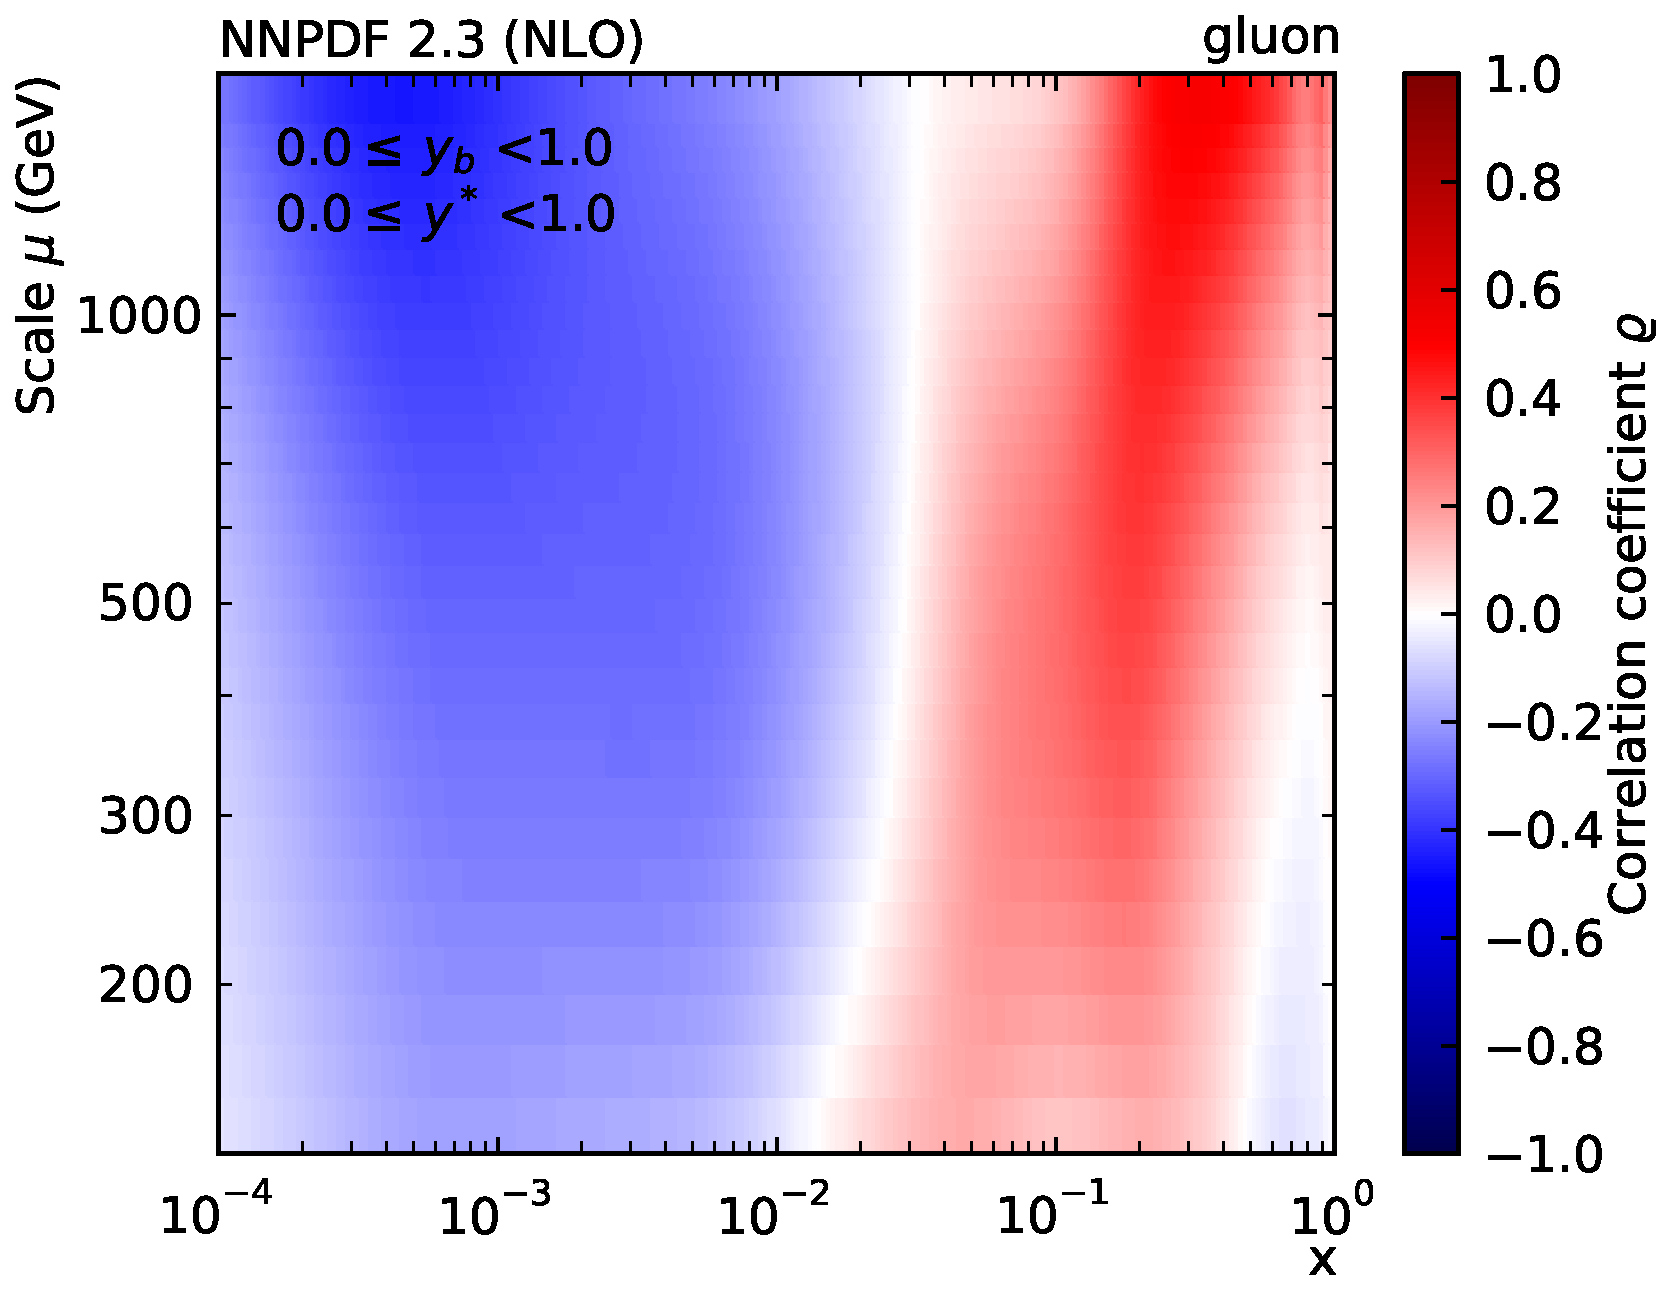
\includegraphics[width=0.49\textwidth]{figures/pdf_constraints/corr_PTMAXEXPYS_YBYS_NLO_FINALBINS_NNPDF23_gluon_ys0_0yb0_0_cl.pdf}\hfill%
  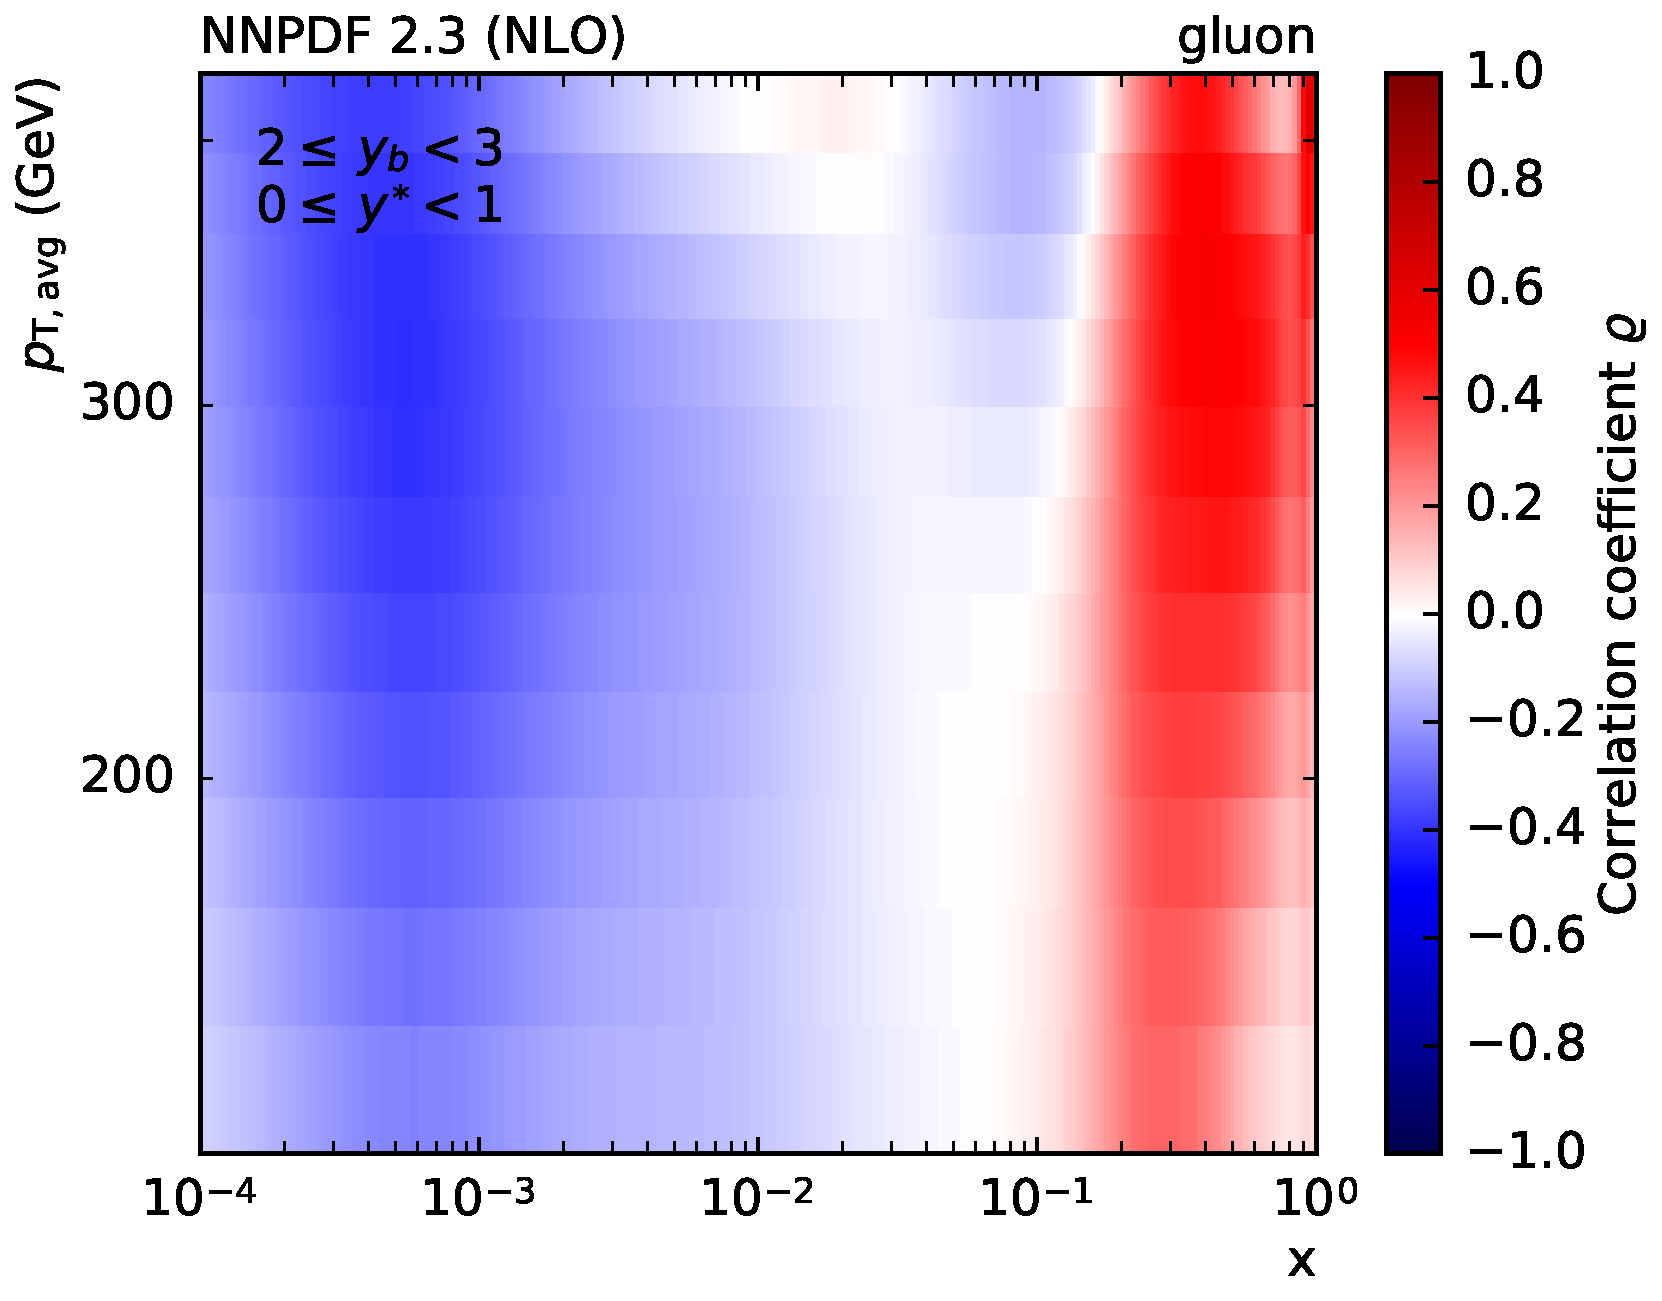
\includegraphics[width=0.49\textwidth]{figures/pdf_constraints/corr_PTMAXEXPYS_YBYS_NLO_FINALBINS_NNPDF23_gluon_ys0_0yb2_0_cl.pdf}
  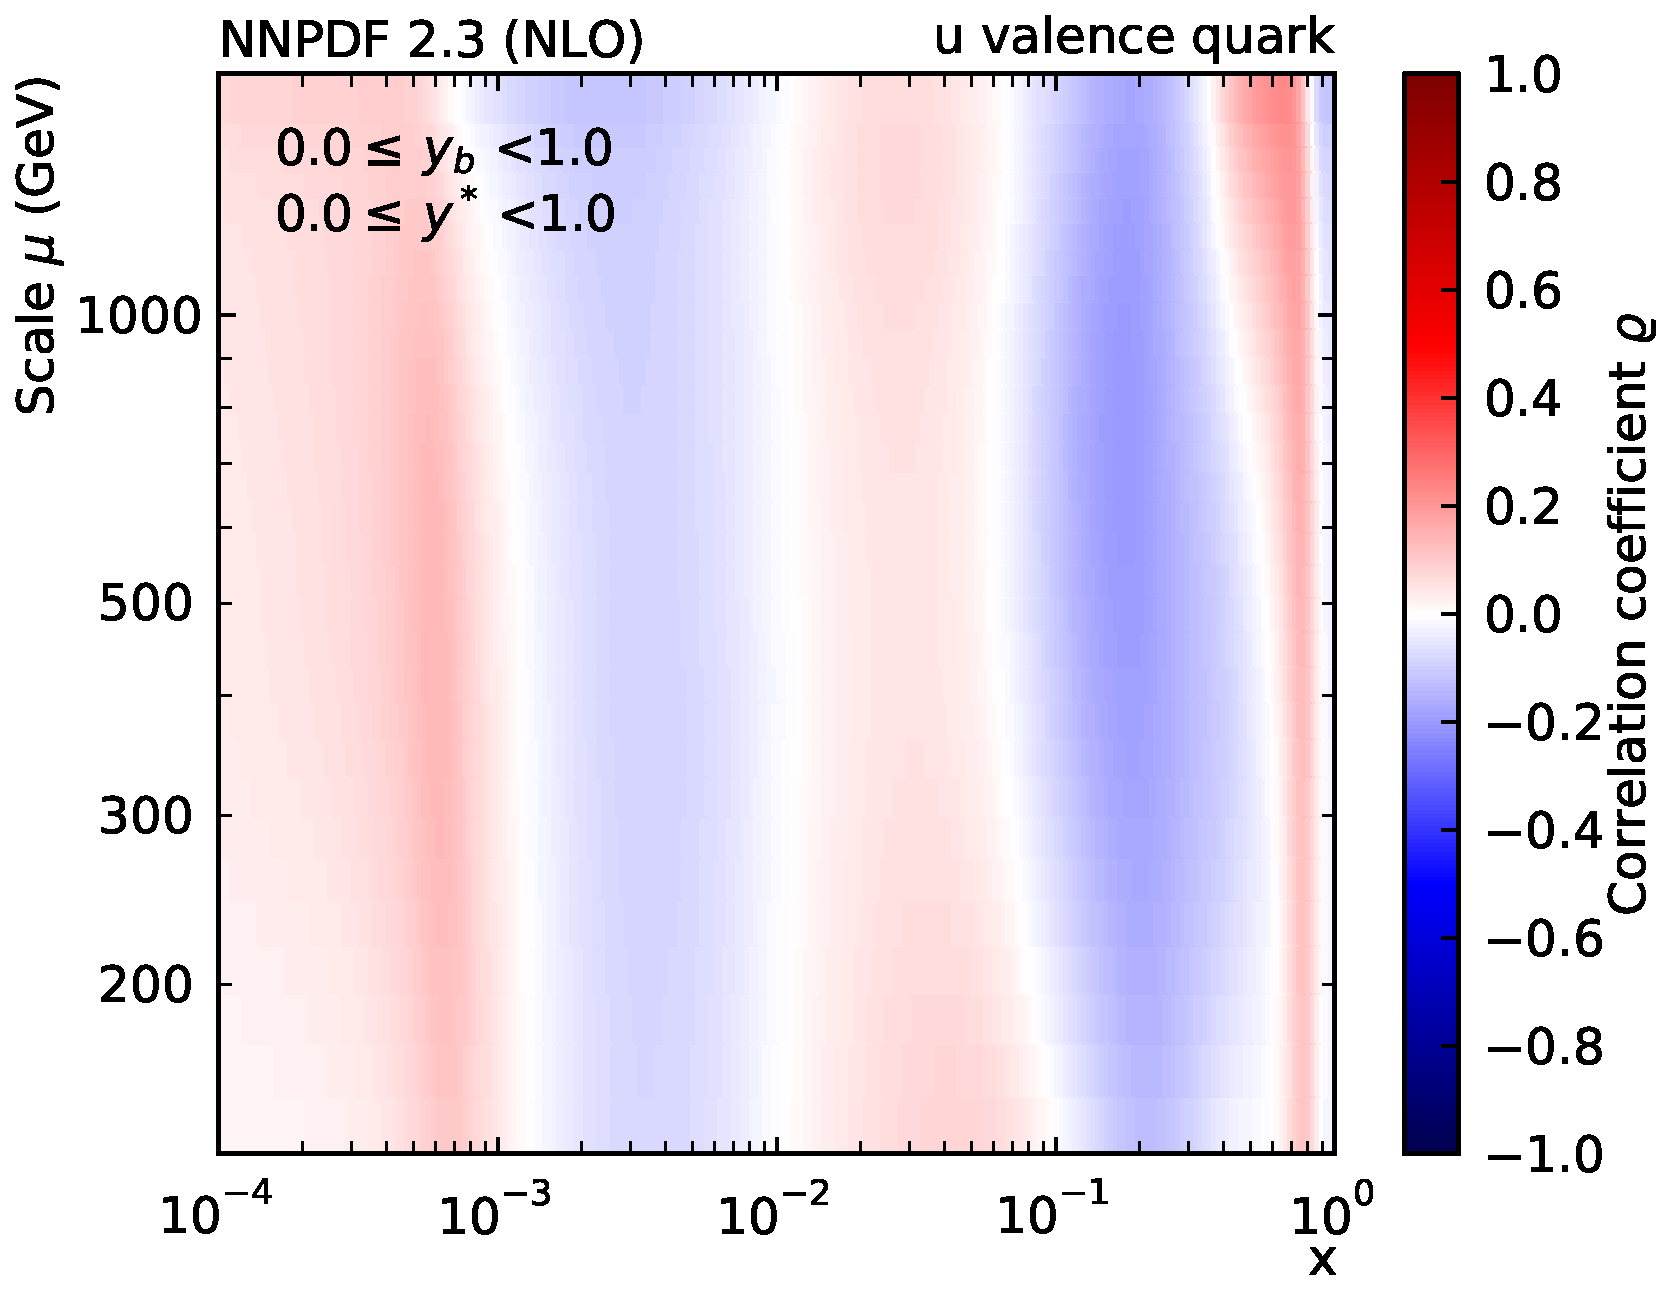
\includegraphics[width=0.49\textwidth]{figures/pdf_constraints/corr_PTMAXEXPYS_YBYS_NLO_FINALBINS_NNPDF23_u_valence_quark_ys0_0yb0_0_cl.pdf}\hfill%
  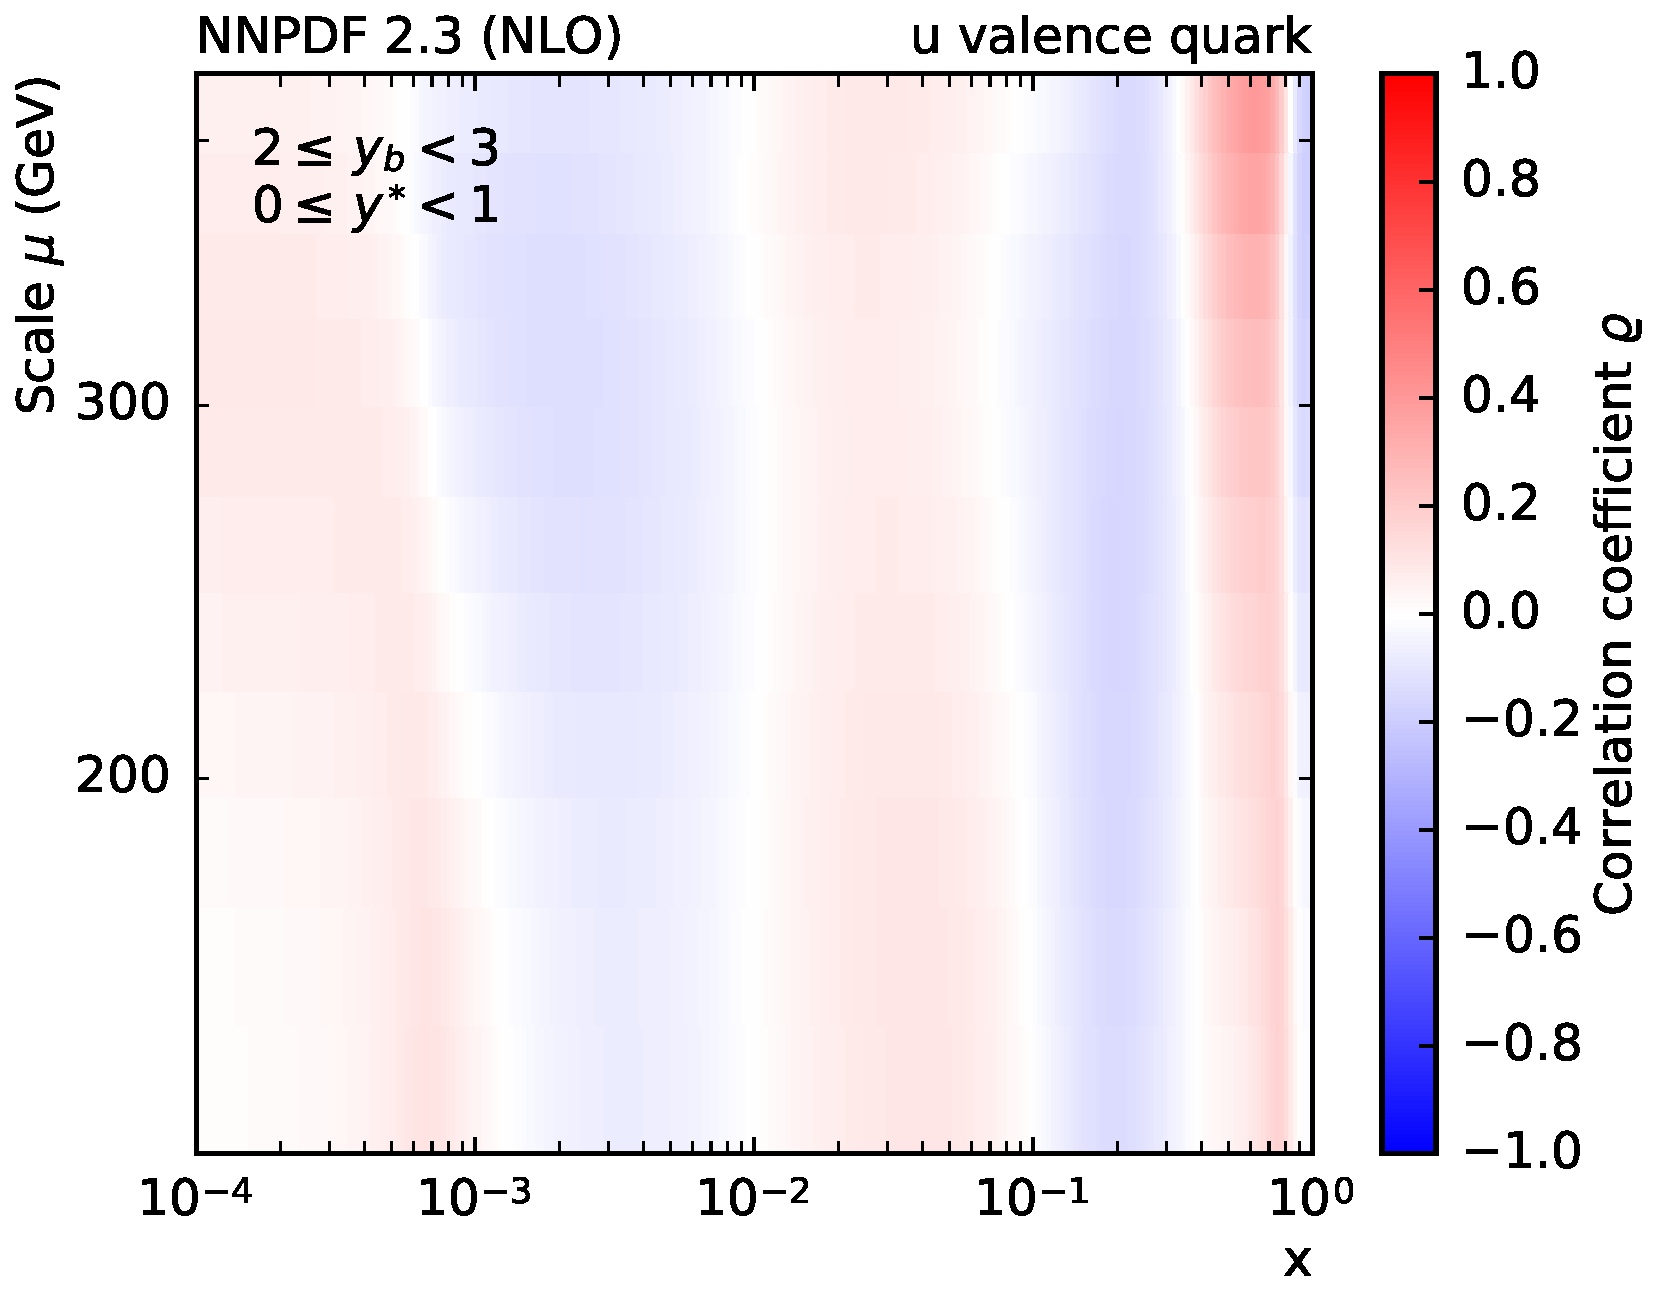
\includegraphics[width=0.49\textwidth]{figures/pdf_constraints/corr_PTMAXEXPYS_YBYS_NLO_FINALBINS_NNPDF23_u_valence_quark_ys0_0yb2_0_cl.pdf}
  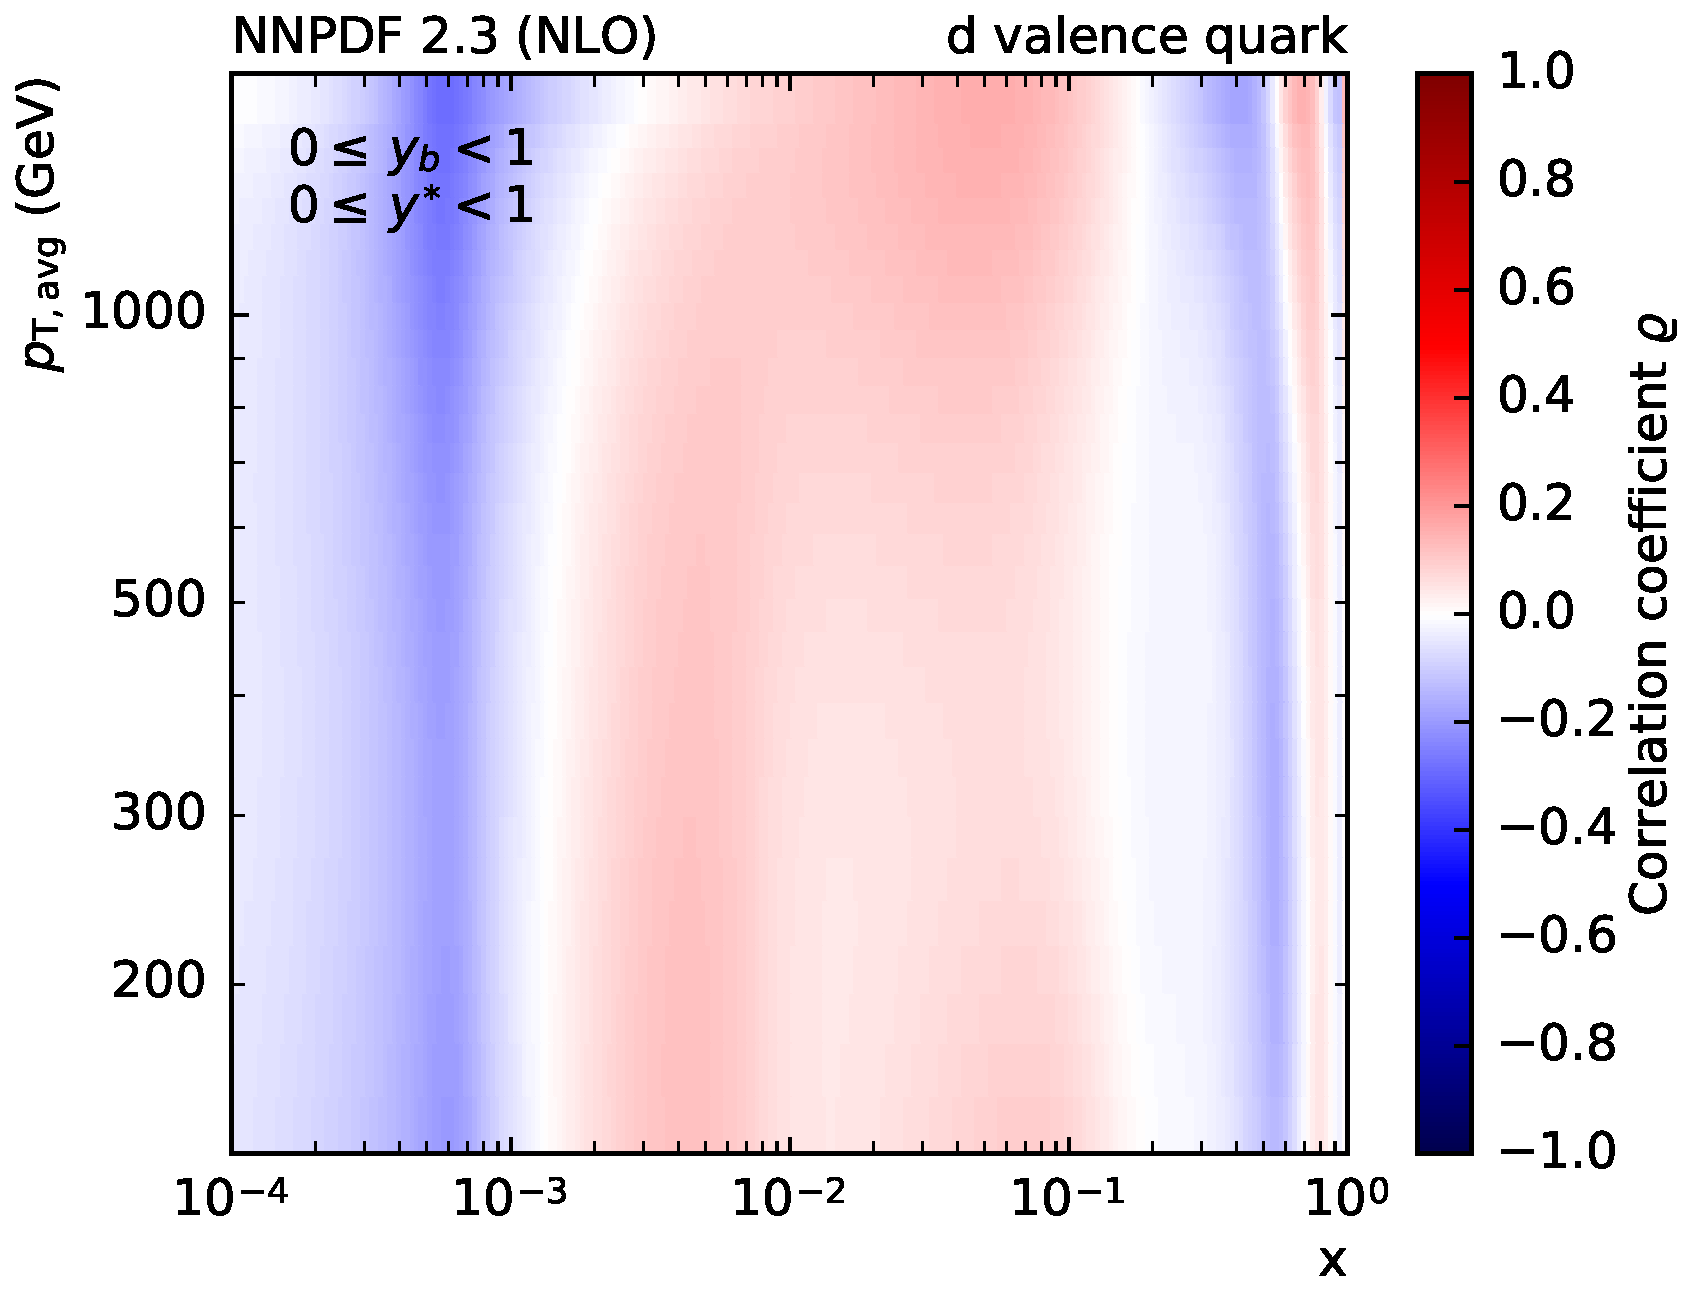
\includegraphics[width=0.49\textwidth]{figures/pdf_constraints/corr_PTMAXEXPYS_YBYS_NLO_FINALBINS_NNPDF23_d_valence_quark_ys0_0yb0_0_cl.pdf}\hfill%
  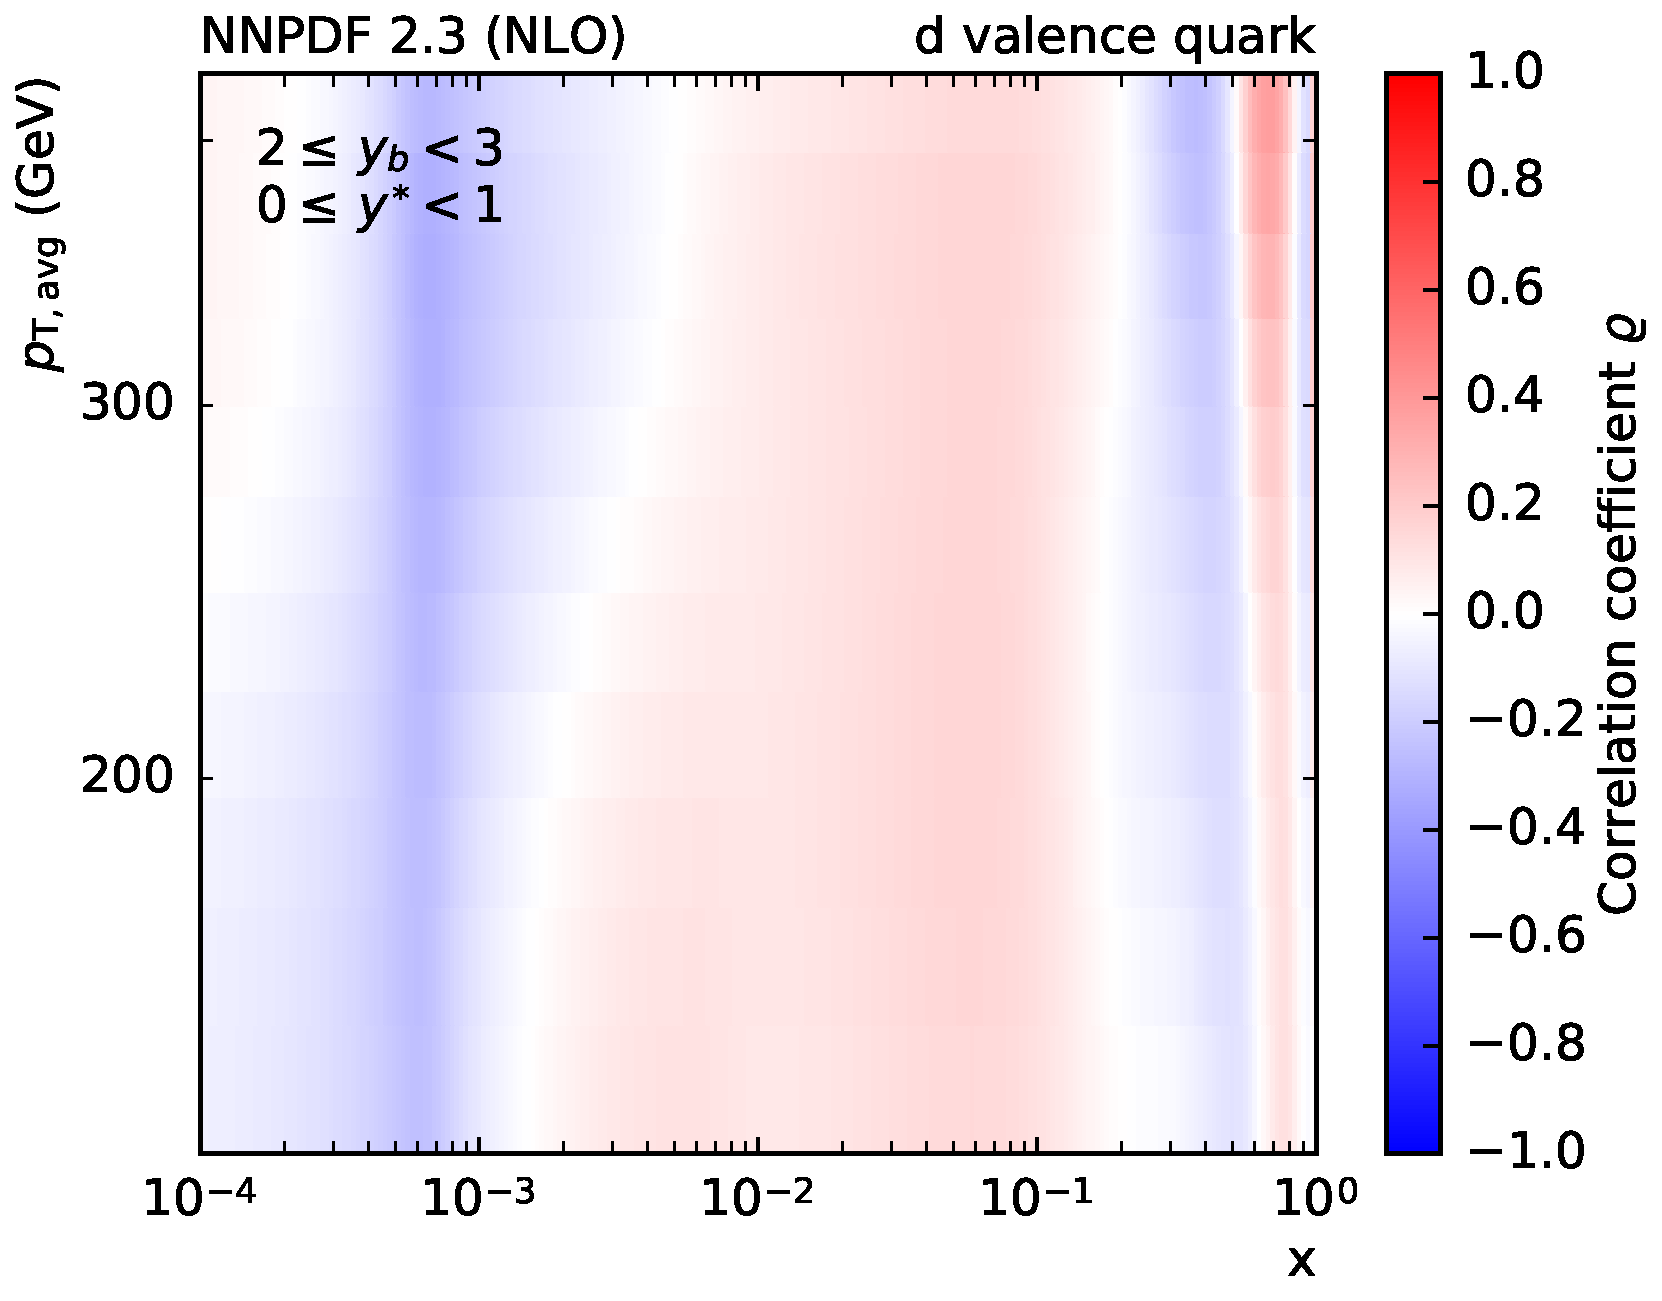
\includegraphics[width=0.49\textwidth]{figures/pdf_constraints/corr_PTMAXEXPYS_YBYS_NLO_FINALBINS_NNPDF23_d_valence_quark_ys0_0yb2_0_cl.pdf}
  \caption[Correlation between dijet cross section and PDFs]{
    The correlation coefficient between the triple-differential dijet cross
    section and the gluon (top row), the u valence quark (middle row),
    and the d valence quark PDFs (bottom row) as a function of the
    momentum fraction $x$ of the proton and the energy scale $\mu$ of
    the hard process. The correlation is shown for the central
    bin $\yboost < 1,\,\ystar < 1$ (left) and for the boosted region $2 \leq
    \yboost < 3$ (right).}
  \label{fig:correlation_pdf_xs_gqq}
\end{figure}

The correlation between the gluon PDF and the dijet cross section is large in
the central bin for \ptavg > \SI{1}{\TeV} and momentum fractions $0.1 < x <
0.5$. In the boosted region there is a large correlation for $\SI{200}{\GeV}
\leq \ptavg < \SI{400}{\GeV}$ and momentum fractions $0.2 < x < 0.7$. In
contrast, the correlation between the dijet cross section and the u valence and
d valence quark PDFs is much smaller, especially in the central region. However,
the correlation in the boosted region is more pronounced, particularly for
highest momentum fractions $x > 0.5$. The results for the remaining bins can be
found in the
Figs~\ref{fig:pdfconstraints_gluon}---\ref{fig:pdfconstraints_sea_quarks}. Based
on the results of the correlation studies, a significant impact of the dijet
cross section is expected by including the dijet cross sections in a PDF fit.

\section{The \xfitter Framework}
\label{section:herafittersetup}

The constraints of the triple-differential dijet measurement on the proton PDFs
are demonstrated by including the cross section measurement in a PDF fit in
combination with inclusive DIS cross sections from the HERA experiments. The
combined HERA-I and HERA-II DIS data were the
basis for the determination of the HERAPDF 2.0 PDF set.

\xfitter~\cite{Alekhin:2014irh} is an open source framework to fit the PDFs to experimental data based
on the DGLAP~\cite{Gribov:1972ri,Altarelli:1977zs,Dokshitzer:1977sg} equations.
To ensure consistency between DIS and QCD calculations, the fits are performed
at NLO as the latter are only available at that order. The DIS cross sections
are calculated by the QCDNUM software~\cite{Botje:2010ay}.

The parametrization used in the PDF fit is based of the
HERAPDF~2.0~\cite{Abramowicz:2015mha} parametrization and introduces additional
terms which were found to better describe the included dijet
measurement. The parametrization of the PDFs is defined at the starting scale
$Q_0^2$
which is set to $Q_0^2 = \SI{1.9}{\GeV \squared}$ and the five independent PDFs
$xu_v(x)$, $xd_v(x)$, $xg(x)$, $x\bar{U}(x)$ and $x\bar{D}(x)$ are parametrized
as follows:
%
\begin{align*}
  xg(x) &= A_g x^{B_g} (1-x)^{C_g} (1 + E_g x^2) - A'_g x^{B'_g} (1-x)^{C'_g} \\
  xu_v(x) &= A_{u_{v}} x^{B_{u_{v}}} (1-x)^{C_{u_{v}}}(1 + D_{u_{v}}x + E_{u_{v}}x^2)\\
  xd_v(x) &= A_{d_v} x^{B_{d_v}} (1-x)^{C_{d_{v}}}\\
  x\bar U(x) &= A_{\bar U} x^{B_{\bar U}} (1-x)^{C_{\bar U}}(1 + D_{\bar U}x)\\
  x\bar D(x) &= A_{\bar D} x^{B_{\bar D}} (1-x)^{C_{\bar D}}
\end{align*}
%
Actually, not all parameters are fitted. The normalization parameters $A_g$,
$A_{u_{v}}$ and $A_{d_{v}}$ are calculated using the QCD sum rules. $B_{\bar
U}=B_{\bar D}$ and $A_{\bar U} = A_{\bar D}(1-f_s)$ ensure the same
normalization for the $\bar u$ and $\bar d$ PDF for the $x \rightarrow 0$
region. The strangeness fraction is set to $f_s = 0.40$. The generalized-mass
variable flavor number scheme as described in~\cite{Thorne:1997ga,Thorne:2006qt}
is used with the strong coupling constant set to $\asmz= 0.1180$.


\subsection{Treatment of Uncertainties in the PDF Fit}
\label{section:treatment_pdf_uncertainties}

The uncertainty of the PDFs is subdivided into three independent sources, which
are evaluated separately and finally added in quadrature to give the total
uncertainty. This procedure was developed by HERAPDF~\cite{Abramowicz:2015mha}
and is followed in this thesis.

\paragraph{Experimental Uncertainties} 
They result from propagated statistical and systematic uncertainties of the data
points and are propagated to the PDFs using the Hessian eigenvector
method~\cite{Pumplin:2001ct}. The Hessian matrix is defined by the second
derivatives of the fitted PDF parameters at the \chisq minimum. The matrix is
diagonalized and the eigenvectors are computed as depicted in
Fig.~\ref{fig:eigenvector_basis_set}. 

\begin{figure}[htb]
  \centering
  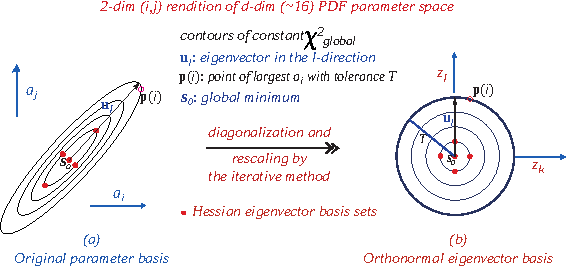
\includegraphics[width=1.0\textwidth]{figures/pdf_constraints/hessianmethod.pdf}
  \caption[Transformation of the parameter basis to the eigenvector basis]
    {Transformation from the original parameter basis to the orthonormal
    eigenvector basis. The uncertainty on the PDFs can be propagated to a
    physical quantity $X$ using these eigenvector PDF sets which are mutually
    uncorrelated. Taken from~\cite{Pumplin:2001ct}.}
    \label{fig:eigenvector_basis_set}
\end{figure}

Using an iterative method, the downwards and upwards variation of each
eigenvector corresponding to $\chisq = \chisq_{\mathrm{min}} + 1$ is calculated.
Since the eigenvectors are orthogonal, the eigenvector variation PDFs correspond
to independent sources of uncertainty on the PDFs. The asymmetric uncertainties
$\Delta X^+$ and $\Delta X^-$ on a quantity of interest $X$ are evaluated as
%
\begin{align*}
  \Delta X^+_{\mathrm{exp}} &= \sqrt{\sum_i^{N_{\mathrm{EV}}} \left[ \max(X_i^{\mathrm{up}}
    -X_0, X_i^{\mathrm{dn}} - X_0, 0)\right]^2}\\
    \Delta X^-_{\mathrm{exp}} &= \sqrt{\sum_i^{N_{\mathrm{EV}}} \left[
    \min(X_i^{\mathrm{up}} - X_0, X_i^{\mathrm{dn}} - X_0,0)\right]^2}\,,
\end{align*}
%
where $X_0$ describes the central prediction and $X_i^{\mathrm{up}}$ and
$X_i^{\mathrm{dn}}$ denote the result using the upwards and downwards variation of
the eigenvector PDF set $i$ of the $N_{\mathrm{EV}}$ eigenvectors in the PDF set.

\paragraph{Model uncertainties} 
The uncertainties of several input parameters in
the PDF fits are combined into one PDF model uncertainty. For the evaluation of
the model uncertainties the following variations on the input parameters are
considered, following the prescription of the HERAPDF 2.0 publication.:
%
\begin{itemize}
\item The assumption is made that the shape of the strange quark PDF follows the
  shape of the down-like sea quark PDF. Thus, the strange quark PDF is not
  fitted but determined as a fraction of the $x\overline{D}$ PDF. The strangeness fraction
  $f_s$, by default set equal to $0.40$, is varied between $0.30$ and $0.50$.
  \item The b-quark mass is set to $\SI{4.5}{\GeV}$ and varied between
  $\SI{4.25}{\GeV}$ and $\SI{4.75}{\GeV}$.
  \item The c-quark mass, set by default to $\SI{1.47}{\GeV}$ is varied between
  $\SI{1.41}{\GeV}$ and $\SI{1.53}{\GeV}$.
  \item The minimum $Q^2$ value for DIS data used in the fit,
    $Q^2_\mathrm{min}=\SI{7.5}{\GeVsq}$, is varied to $Q^2_\mathrm{min} =
    \SI{5.0}{\GeV\squared}$ and $Q^2_\mathrm{min} = \SI{10.0}{\GeV\squared}$.
\end{itemize}
%
The model uncertainty is evaluated in the same way as the PDF eigenvectors.
The variation of each input parameter is treated as an independent variation
leading to the definition of the asymmetric model uncertainty as:

\begin{align*}
  \Delta X^+_{\mathrm{mod}} &= \sqrt{\sum_i^{N_{\mathrm{par}}} \left[ \max(X_i^{\mathrm{up}}
    -X_0, X_i^{\mathrm{dn}} - X_0, 0)\right]^2}\\
    \Delta X^-_{\mathrm{mod}} &= \sqrt{\sum_i^{N_{\mathrm{par}}} \left[ \min(X_i^{\mathrm{up}} - X_0, X_i^{\mathrm{dn}} - X_0,0)\right]^2}
\end{align*}

\paragraph{Parametrization uncertainty}

To estimate the influence of the initial PDF parametrization on the fit result, a
more flexible function form is used. Using the general
parametrizations for the gluon PDF $xg(x)$ and the quark PDFs $xf(x)$
%
\begin{align*}
   xg(x) &= A_g x^{B_g} (1-x)^{C_g} (1  + D_g x + E_g x^2) - A'_g x^{B'_g} (1-x)^{C'_g}\\
\intertext{and}
   xf(x) &= A_{f}  x^{B_{f}} (1-x)^{C_{f}} (1 + D_{f}x + E_{f}x^2),
\end{align*}
%
it is studied if the inclusion of additional parameters in the fit yields
different results. Each parameter is succesively added in the PDF fit and the
envelope of all changes to the PDF shape is combined into one parametrization
uncertainty. Furthermore, the variation of the starting scale $Q_0^2$ to
\SI{1.6}{\GeV\squared} and \SI{2.2}{\GeV\squared} is treated as an 
parametrization variation.

\begin{align*}
  \Delta X^+_{\mathrm{par}} &= \max_{i}^{n} \left[ X^i - X^0, 0 \right]\\
  \Delta X^-_{\mathrm{par}} &= \max_{i}^{n} \left[ X^0 - X^i, 0 \right]
\end{align*}


\subsection{Definition of the Goodness-of-Fit Estimator}
\label{sec:chi2_definition}

The minimization procedure of the PDF fit is using a least-squares method. The \chisq is
calculated with the data points $D_i$ and the theoretical prediction $T_i$. The
$K$  correlated systematic uncertainties $\beta_{k}$ are treated using nuisance parameters
$_k$ in the fit, which are applied to the theoretical prediction, to avoid the bias from
multiplicative data uncertainties, see~\cite{Lyons:1989gh}. The \chisq is
defined as

\begin{align*}
  \chi^2 = &\sum_{ij}^N \left(D_i - T_i - \sum_k^K r_k \beta_{ik}\right) \mathrm{C}_{ij}^{-1}
  \left(D_j - T_j - \sum_k^K r_k \beta_{jk} \right) + \sum_k^K r_k^2\\
  &+ \sum_j \ln \frac{\Delta_{i,\mathrm{stat}}^2 D_j T_j + \Delta_{i,\mathrm{uncor}}^2 T_i^2}{\left( \Delta_{i,\mathrm{stat}}^2 + \Delta_{i,\mathrm{uncor}}^2 \right) D_i^2}
  \label{chi2_nuisance}
\end{align*}

where $C_{ij}^{-1}$ is the inverse covariance matrix of the uncorrelated
systematic and statistical uncertainties and $\Delta_\mathrm{stat}$ and
$\Delta_\mathrm{uncor}$ are the diagonal elements of the statistical and
uncorrelated uncertainty. More information can be found
in~\cite{Alekhin:2014irh,Abramowicz:2015mha}. An advantage of such a \chisq
definition with nuisance parameters is the possibility to study the pulls of
each systematic source after the fit.

\subsection{Treatment of Systematic Uncertainties}
\label{section:cmsdatauncertainties}

% The dominant source of experimental uncertainty is due to the jet energy scale.
% This uncertainty is split into 25 sources which are correlated among themselves
% but uncorrelated to each other.
%
Since the correlated sources of uncertainty are treated using nuisance
parameters in the \chisq formula, the pull of each source can be examined.
Tab.~\ref{tab:pdfconstraints:nuisance} shows the 27 sources of systematic
uncertainty and their pulls. Most of the systematic sources shift by less than
one standard deviation. Three sources exhibit larger shifts. While this not
surprising due to the gaussian distributution of the pulls, no unambiguous
reason for their behaviour could be identified. However, the size of these
uncertainty sources is rather small compared to the dominant sources of
uncertainty so that no significant influence on the fit is expected.

\begin{table}[htbp]
  \caption[Nuisance parameters determined in PDF fit]{Nuisance parameters
  obtained by the PDF fit to HERA-II DIS data and the CMS dijet cross
  sections. Most of the pulls cause shifts by less than a standard deviation.}
  \label{tab:pdfconstraints:nuisance}
  \centering
  \begin{tabular}{lrlr}
    \toprule
    Systematic source        & Shift in $\sigma$ & Systematic source        & Shift in $\sigma$\rbthm\\\midrule
    \textsc{AbsoluteScale}   & -0.18             & \textsc{RelativeFSR}     & 2.45  \rbtrr\\
    \textsc{AbsoluteStat}    & -0.37             & \textsc{RelativeStatEC2} & -0.38  \rbtrr\\
    \textsc{AbsoluteMPFBias} & -0.21             & \textsc{RelativeStatHF}  & 0.03  \rbtrr\\
    \textsc{Fragmentation}   & -0.06             & \textsc{RelativeStatFSR} & -0.06  \rbtrr\\
    \textsc{SinglePionECAL}  & 0.13              & \textsc{PileUpDataMC}    & -0.03  \rbtrr\\
    \textsc{SinglePionHCAL}  & -0.85             & \textsc{PileUpPtRef}     & -1.05  \rbtrr\\
    \textsc{FlavorQCD}       & 1.26              & \textsc{PileUpPtBB}      & 0.89  \rbtrr\\
    \textsc{RelativeJEREC1}  & 0.54              & \textsc{PileUpPtEC1}     & -0.73  \rbtrr\\
    \textsc{RelativeJEREC2}  & -0.26             & \textsc{PileUpPtEC2}     & 0.03  \rbtrr\\
    \textsc{RelativeJERHF}   & 0.04              & \textsc{PileUpPtHF}      & 0.00  \rbtrr\\
    \textsc{RelativePtBB}    & -0.14             & \textsc{nperr}           & -2.02  \rbtrr\\
    \textsc{RelativePtEC1}   & -1.03             & \textsc{jererr}          & 0.36  \rbtrr\\
    \textsc{RelativePtEC2}   & -2.49             & \textsc{lumi}            & 0.62  \rbtrr\\
    \textsc{RelativePtHF}    & 0.01              &                          & \rbtrr\\
    \bottomrule
  \end{tabular}
\end{table}

\section{Constraints on PDFs of the Triple-Differential Dijet Cross Section}
\label{section:cmsjets2011_pdfconstraints}

The quality of the fit with and without including the dijet measurement is
reported in Table~\ref{tab:fit:results}. The partial \chisq per data point for
each data set as well the \chisq per \ndof for all data sets demonstrate
the compatibility of the CMS dijet measurement and the DIS data from the HERA
experiments. 

\begin{table}[htbp]
\small
\setlength\tabcolsep{3.5pt} 
  \caption[Fit quality in the HERA DIS and combined fit]{The Partial \chisq's  for each data set in the HERA DIS (middle
    section) or the combined fit including the triple-differential dijet data
    (right section) are shown.
    \ndata is the number of data points available for the determination of
    the 13 parameters. The bottom two lines show the total \chisq and
    \chisqndof. The difference between the sum of all
    \chipsq and the total \chisq for the combined fit is attributed to
    the nuisance parameters.}
  \label{tab:fit:results}
  \centering
  \begin{tabular}{lrrcrc}
    \toprule
    \multicolumn{2}{c}{} &
    \multicolumn{2}{c}{HERA data} &
    \multicolumn{2}{c}{HERA \& CMS data}\rbtrr\\\cmidrule(l){3-6}
    data set &
    \multicolumn{1}{c}{\ndata} &
    \multicolumn{1}{c}{\chipsq} &
    \multicolumn{1}{c}{\chipsqndata} &
    \multicolumn{1}{c}{\chipsq} &
    \multicolumn{1}{c}{\chipsqndata}\rbthm\\\midrule
    CC HERA-I+II H1-ZEUS e-p.                                   & 42  & 54.96  & 1.31  & 54.8   & 1.30 \rbtrr\\
    CC HERA-I+II H1-ZEUS e+p.                                   & 39  & 38.36  & 0.98  & 38.16  & 0.98 \rbtrr\\
    NC HERA-I+II H1-ZEUS e-p.                                   & 159 & 218.2  & 1.37  & 218.99 & 1.38 \rbtrr\\
    NC HERA-I+II H1-ZEUS e+p. $E_{\mathrm{p}} = \SI{460}{\GeV}$ & 187 & 206.83 & 1.11  & 207.62 & 1.11 \rbtrr\\
    NC HERA-I+II H1-ZEUS e+p. $E_{\mathrm{p}} = \SI{575}{\GeV}$ & 234 & 200.8  & 0.86  & 203.07 & 0.87 \rbtrr\\
    NC HERA-I+II H1-ZEUS e+p. $E_{\mathrm{p}} = \SI{820}{\GeV}$ & 63  & 61.14  & 0.97  & 62.73  & 1.00 \rbtrr\\
    NC HERA-I+II H1-ZEUS e+p. $E_{\mathrm{p}} = \SI{920}{\GeV}$ & 332 & 370.18 & 1.12  & 387.34 & 1.17 \rbtrr\\
    \textsc{CMS Triple-Differential Dijets}                     & 111 & ---    & ---   & 90.57  & 0.82
    \rbtrr\\\bottomrule
    data set(s) & \ndof &
    \multicolumn{1}{c}{\chisq} &
    \multicolumn{1}{c}{\chisqndof} &
    \multicolumn{1}{c}{\chisq} &
    \multicolumn{1}{c}{\chisqndof}\rbthm\\\midrule
    HERA data                       & 1042 & 1203.86 & 1.16  &  --- &  --- \rbtrr\\
    HERA \& CMS data                & 1164 &    --- &  --- & 1330.61 & 1.15 \rbtrr\\
    \bottomrule
  \end{tabular}
\end{table}

The resulting PDF for the gluon, u valence, d valence and sea quark for a fit
with and without the CMS dijet data are arranged next to each other in the
Figs.~\ref{fig:pdfconstraints:split:gluonqsea:19}--\ref{fig:pdfconstraints:split:dvaluval:19}
while Fig.~\ref{fig:pdfconstraints:direct:19} and
Fig.~\ref{fig:pdfconstraints:direct:10000} give a direct comparison of the PDFs
with total uncertainties. The uncertainty breakdown in
Fig.~\ref{fig:pdfconstraints:split:gluonqsea:19} reveals the large impact of
the dijet data. The uncertainty of the gluon PDF is reduced over almost the
whole range in $x$. The experimental uncertainty is drastically reduced in the
high-$x$ region above $x \gtrsim 0.1$. Less pronounced changes are visible in
the low-$x$ gluon PDF in which most of the uncertainty changes can be attributed
to the parameterization uncertainty. The large changes of uncertainties come
along with a noticeably change of the high-$x$ gluon PDF shape. The gluon PDF is
much harder compared to the fit with HERA DIS data alone. Similar changes were
observed before, \eg in~\cite{Khachatryan:2014waa}.

The changes of the sea quark PDF, defined as $x\Sigma=2(x\overline U + x
\overline D + x\overline s)$, are much less pronounced.
Only the parametrization uncertainty is clearly reduced in the high-$x$ region.
The u valence and d valence quark PDFs also show uncertainty reductions over
the whole $x$-range. The uncertainty decrease of the experimental uncertainty is
sizable for high-$x$, while the main differences result from the parametrization
uncertainty, which is signifcant for the fit with HERA DIS data alone, but
almost completely vanishes in the fit including the CMS dijet data.

In contrast to the previous figures, Fig.~\ref{fig:pdfconstraints:direct:10000}
shows the PDFs after the evolution to the scale $Q^2 = \SI{10000}{\GeV \square}$
which is close to the scale of the measurement. The PDFs exhibit the same
features compared to the starting scale $Q_0$, but even more pronounced.
Finally, an overview of of the gluon, sea, u valence and d valence quark PDFs is
given in Fig.~\ref{fig:pdfconstraints:overview:19}. 

The large impact of the data on the PDFs is partly caused by the limited
precision of the fit using HERA DIS data alone. In a global PDF fit, constraints
from other measurements already improve the PDFs, so that not such a strong
impact is expected. However, it was shown in Sec.~\ref{sec:nlo_comparisons} that
predictions using the global PDF sets do not describe the data in certain phase
space regions. There, also improvements of the global PDF sets are expected.

\begin{figure}[tbp]
  \centering
  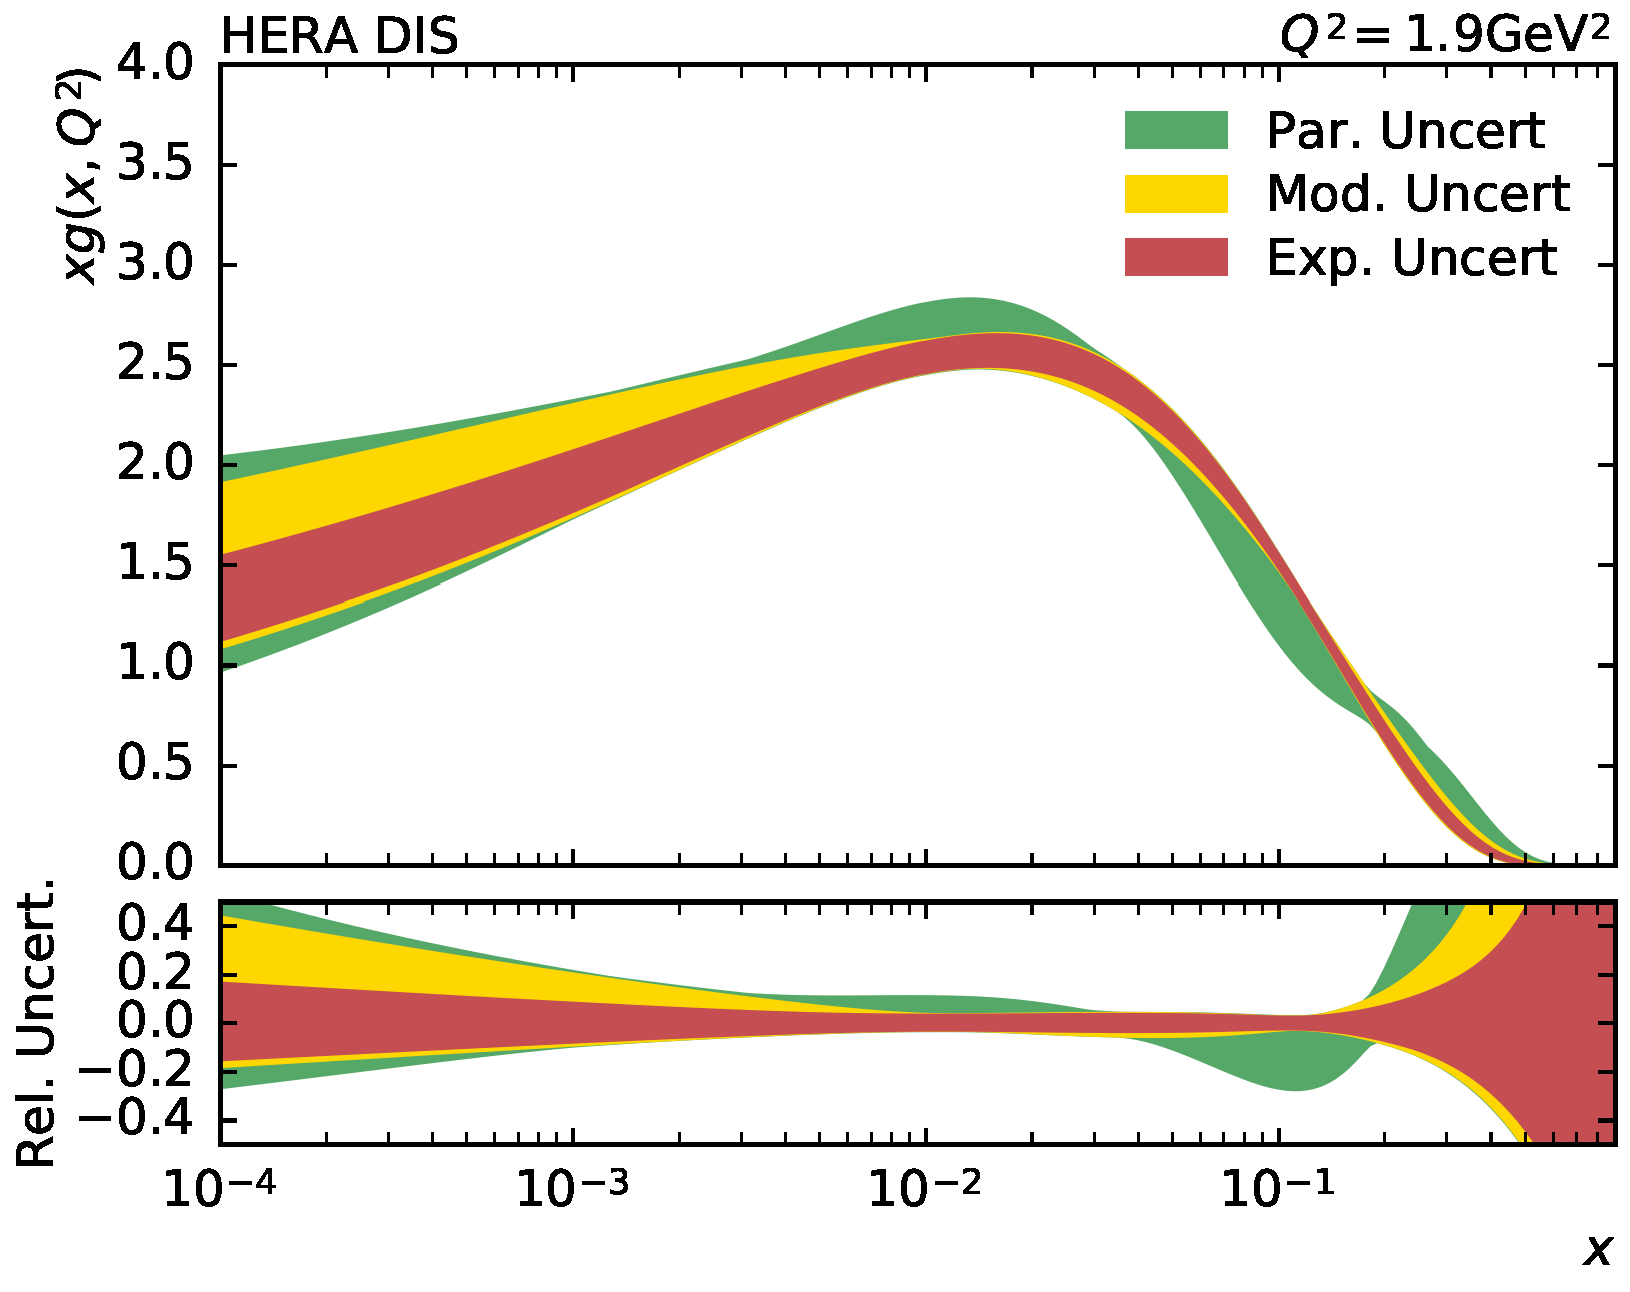
\includegraphics[width=0.48\textwidth]{figures/pdf_constraints/pdfcomp_HFTD_HERA_0_1.9.pdf}\hfill%
  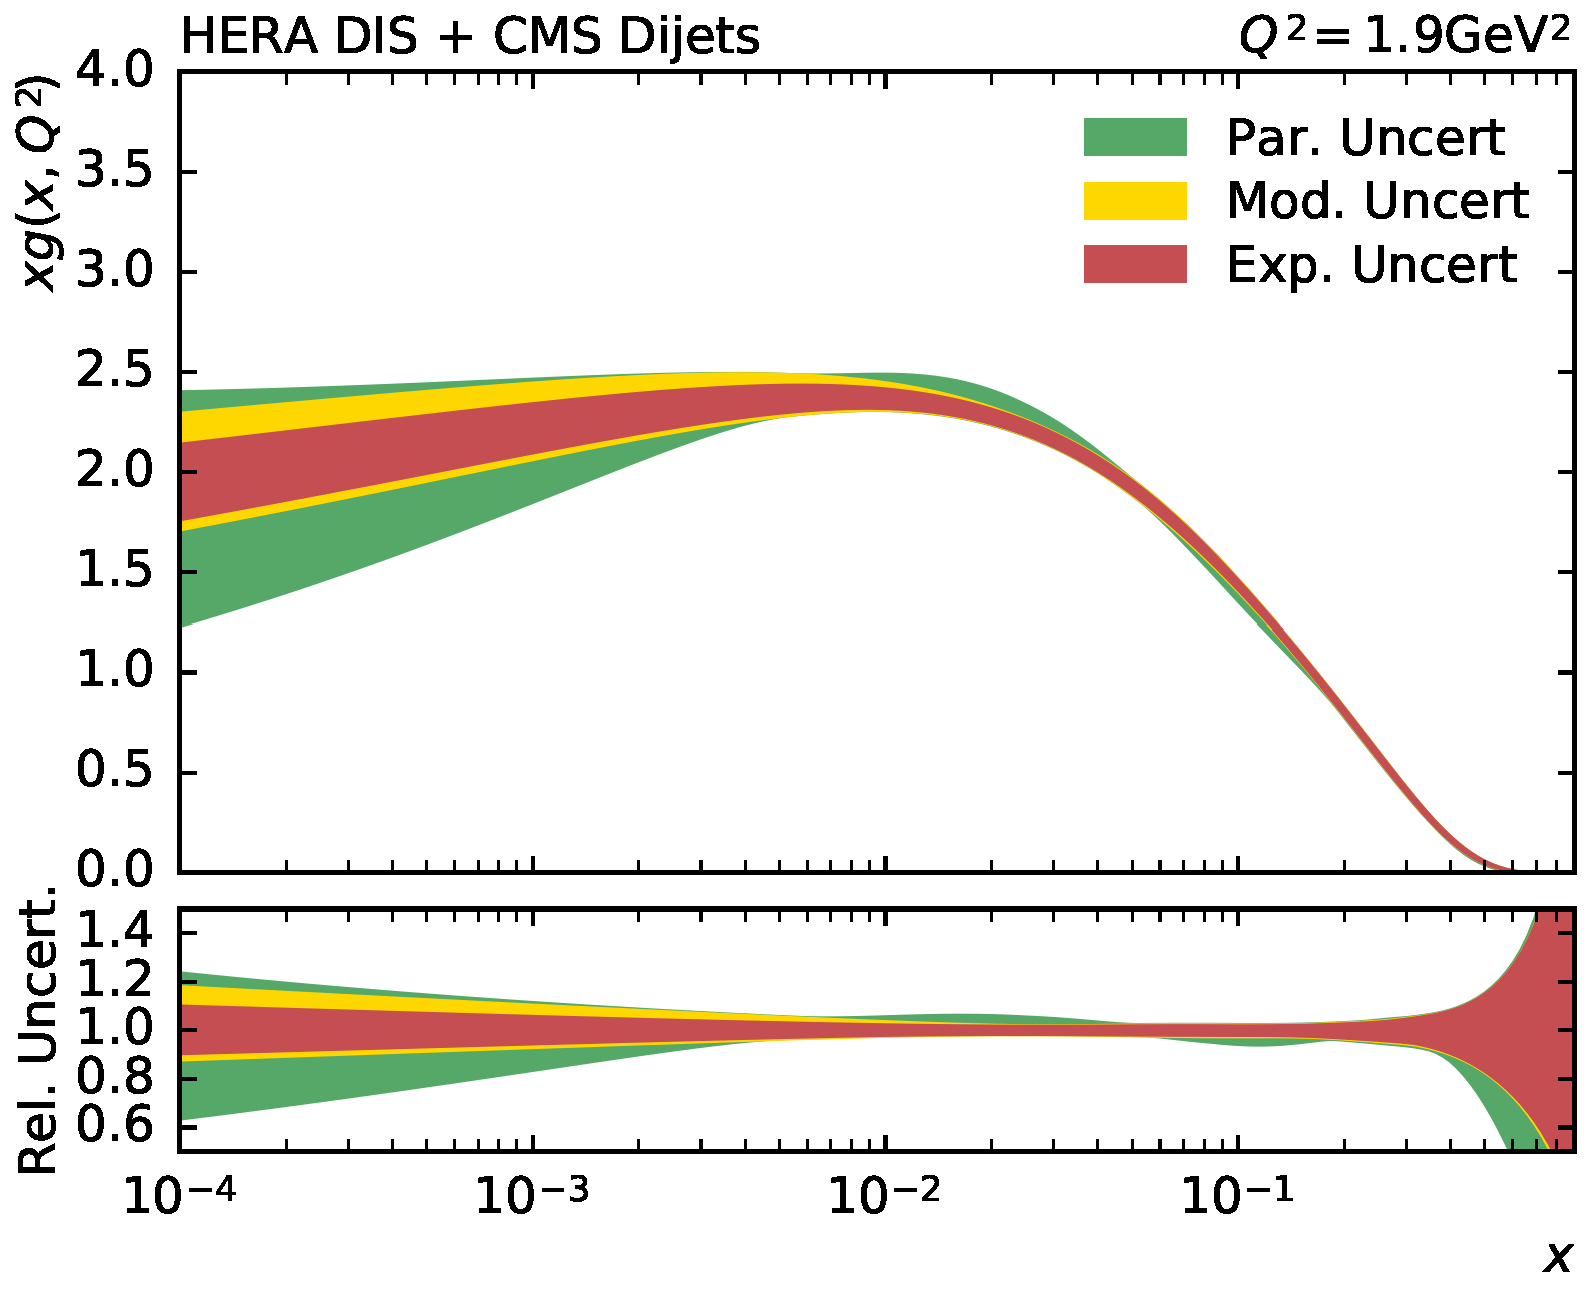
\includegraphics[width=0.48\textwidth]{figures/pdf_constraints/pdfcomp_HFTD_HERACMSTDJETS_0_1.9.pdf}
  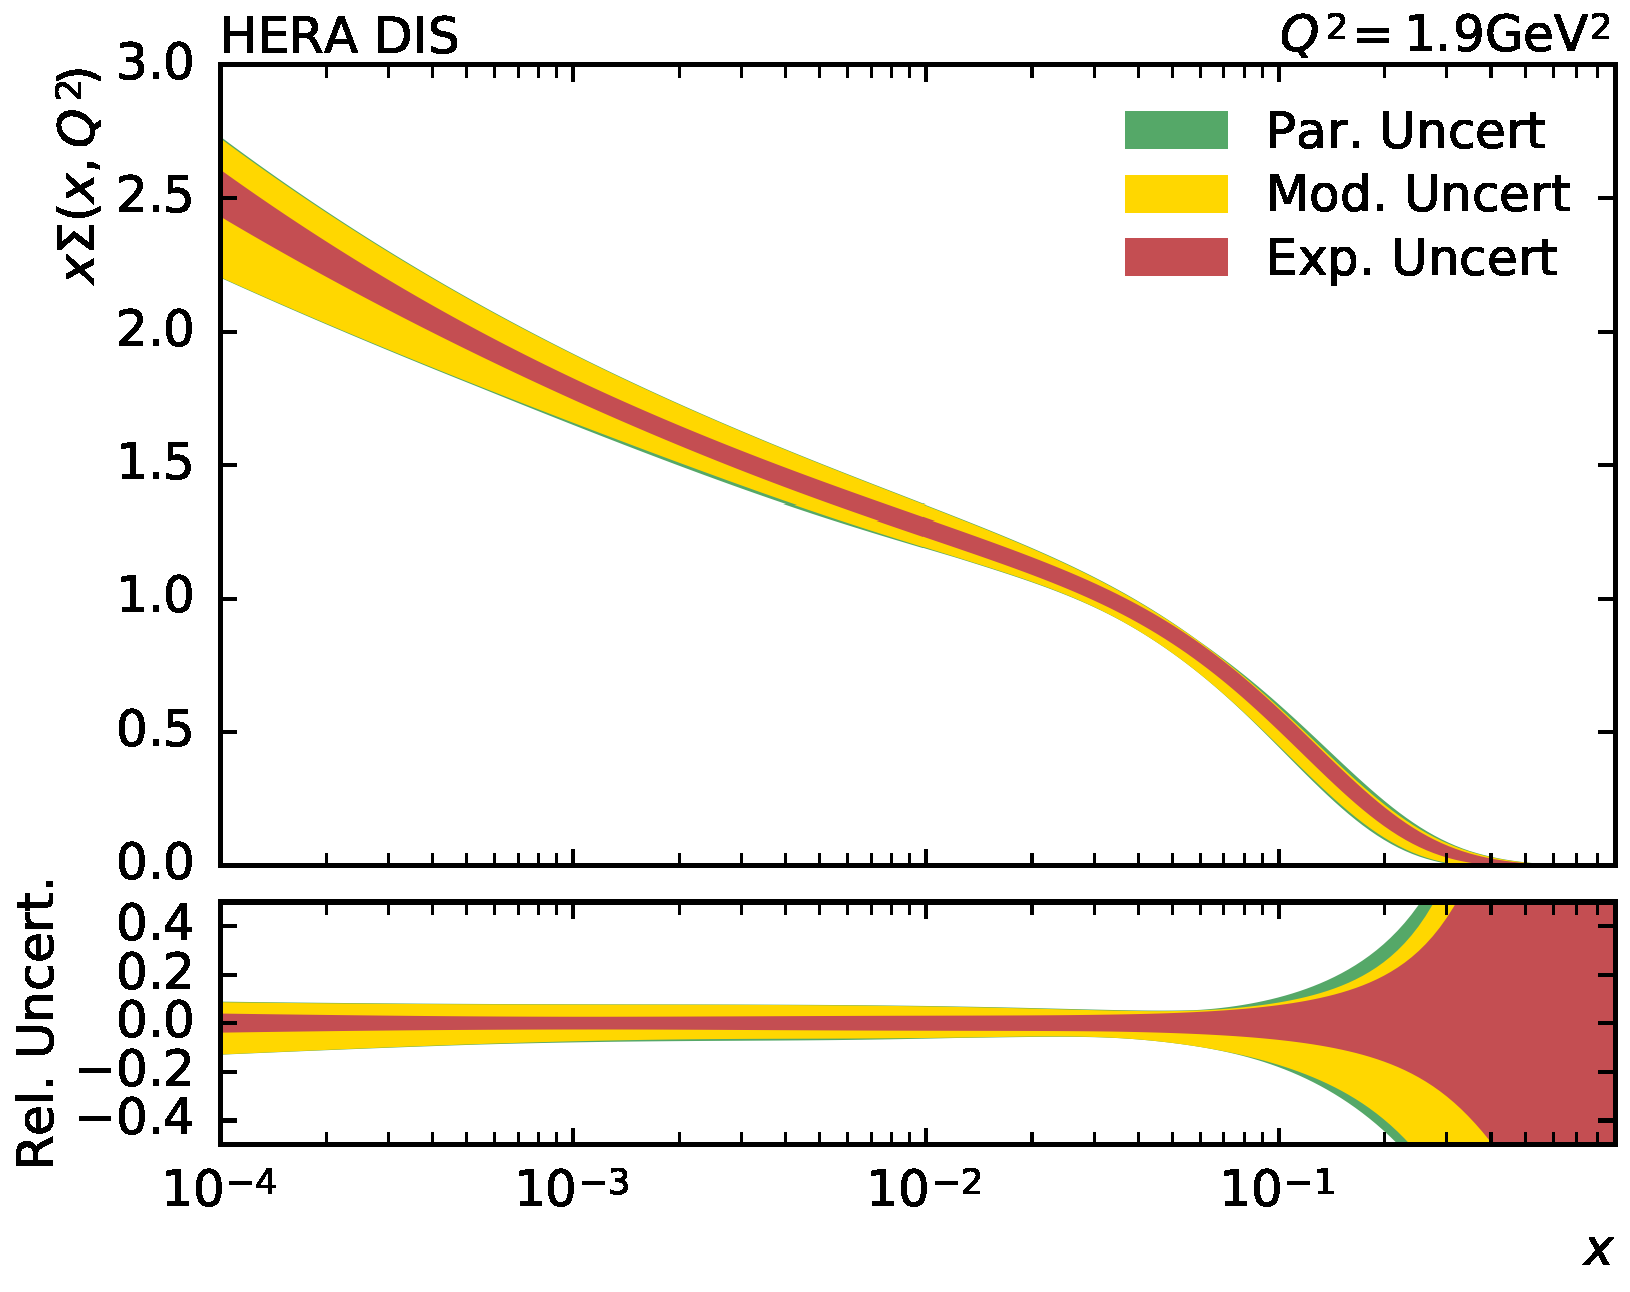
\includegraphics[width=0.48\textwidth]{figures/pdf_constraints/pdfcomp_HFTD_HERA_9_1.9.pdf}\hfill%
  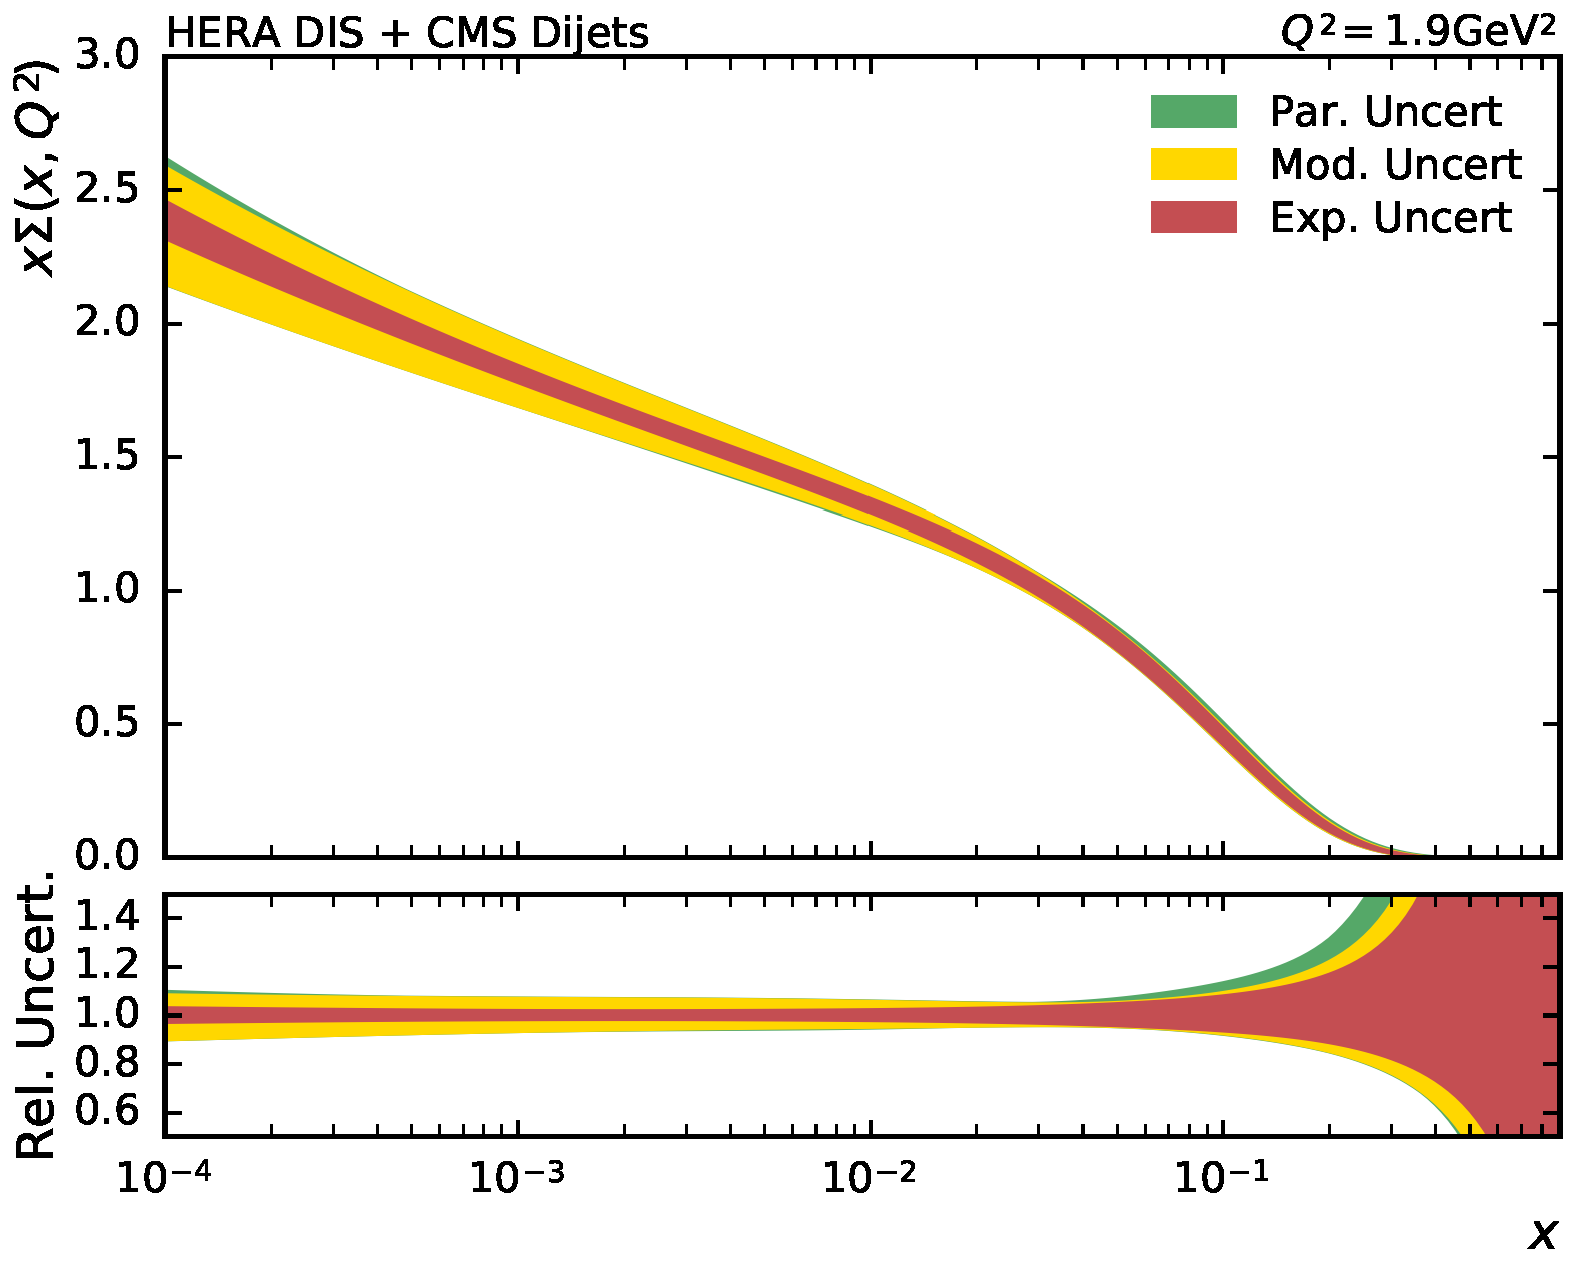
\includegraphics[width=0.48\textwidth]{figures/pdf_constraints/pdfcomp_HFTD_HERACMSTDJETS_9_1.9.pdf}
  \caption[The gluon and sea quark PDFs]{The gluon (top) and sea quark (bottom) PDFs as a function of $x$ as
  derived from HERA inclusive DIS data alone (left) and in combination with
  the CMS dijet data (right). The PDFs are shown at the starting scale $Q^2 =
  \SI{1.9}{\GeV \squared}$. The experimental (inner band), model (middle band)
  and parametrization uncertainties (outer band) are added quadratically to give
  the total uncertainty.}
  \label{fig:pdfconstraints:split:gluonqsea:19}
\end{figure}

\begin{figure}[tbp]
  \centering
  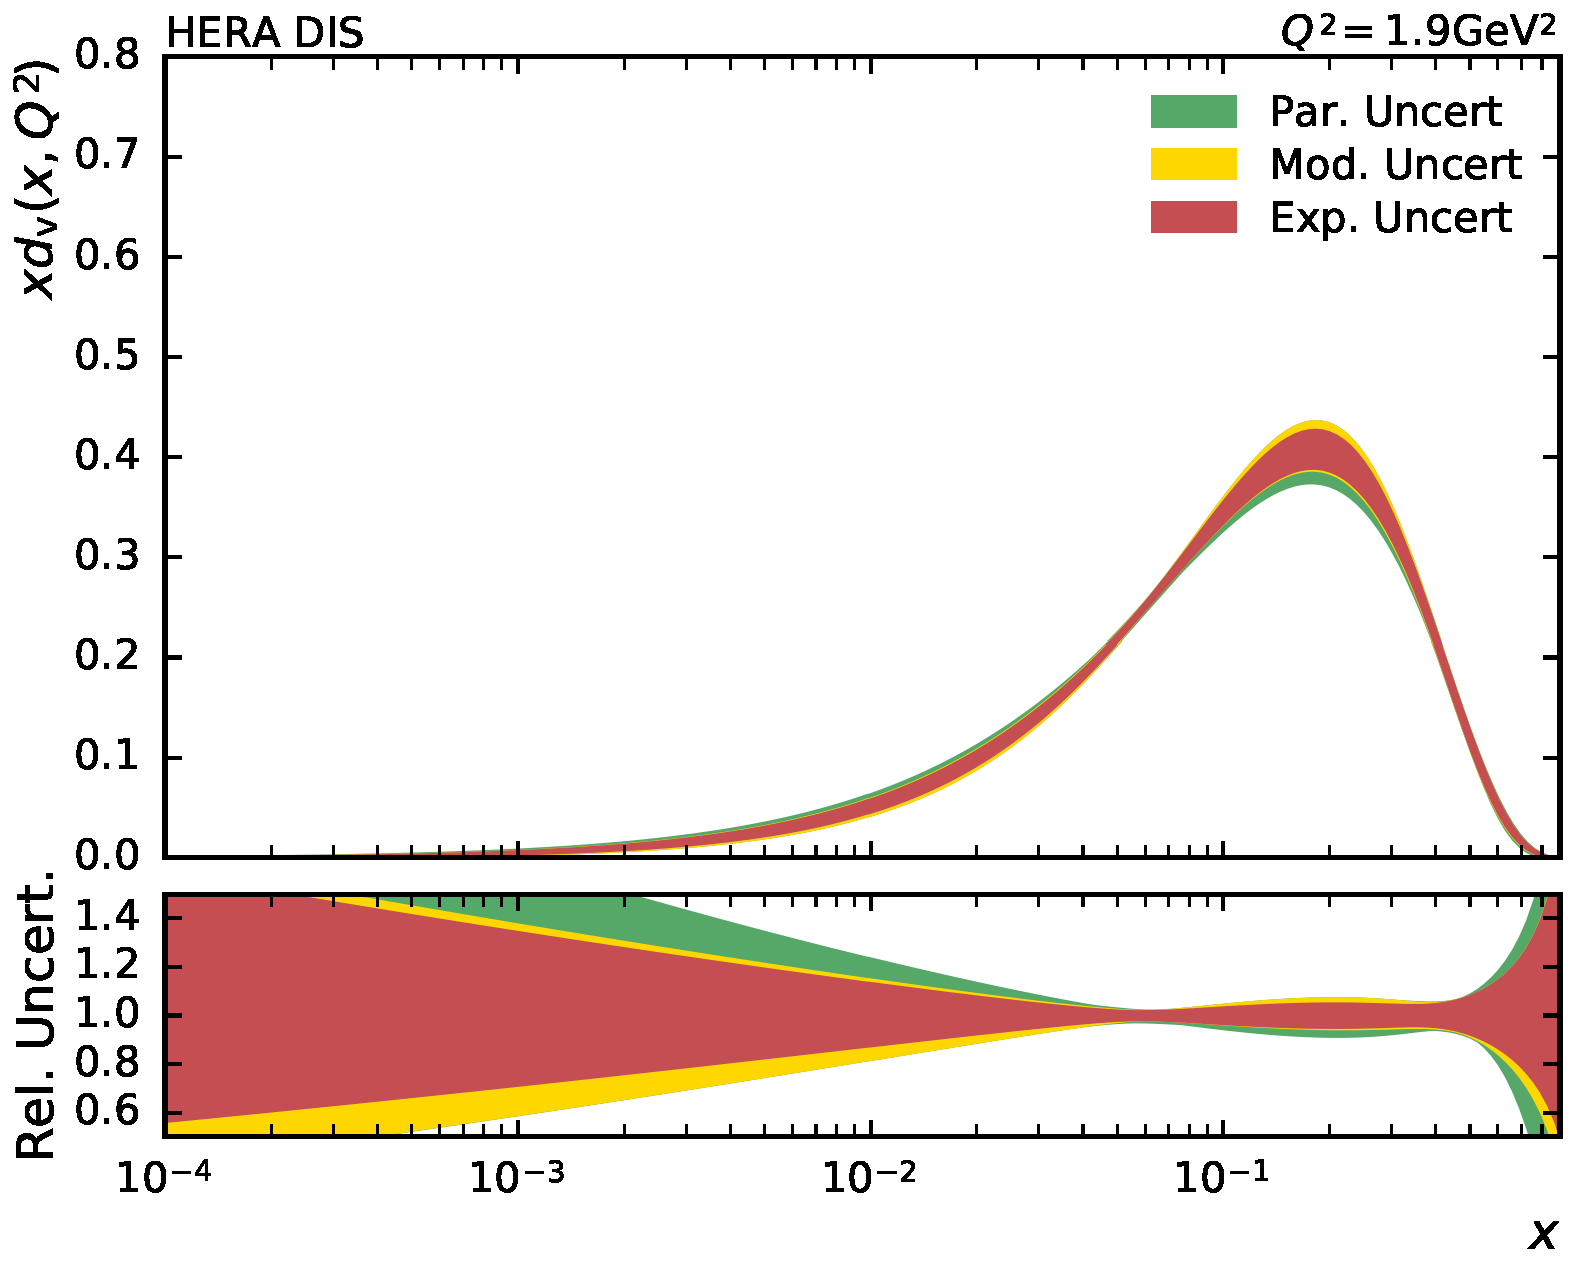
\includegraphics[width=0.48\textwidth]{figures/pdf_constraints/pdfcomp_HFTD_HERA_7_1.9.pdf}\hfill%
  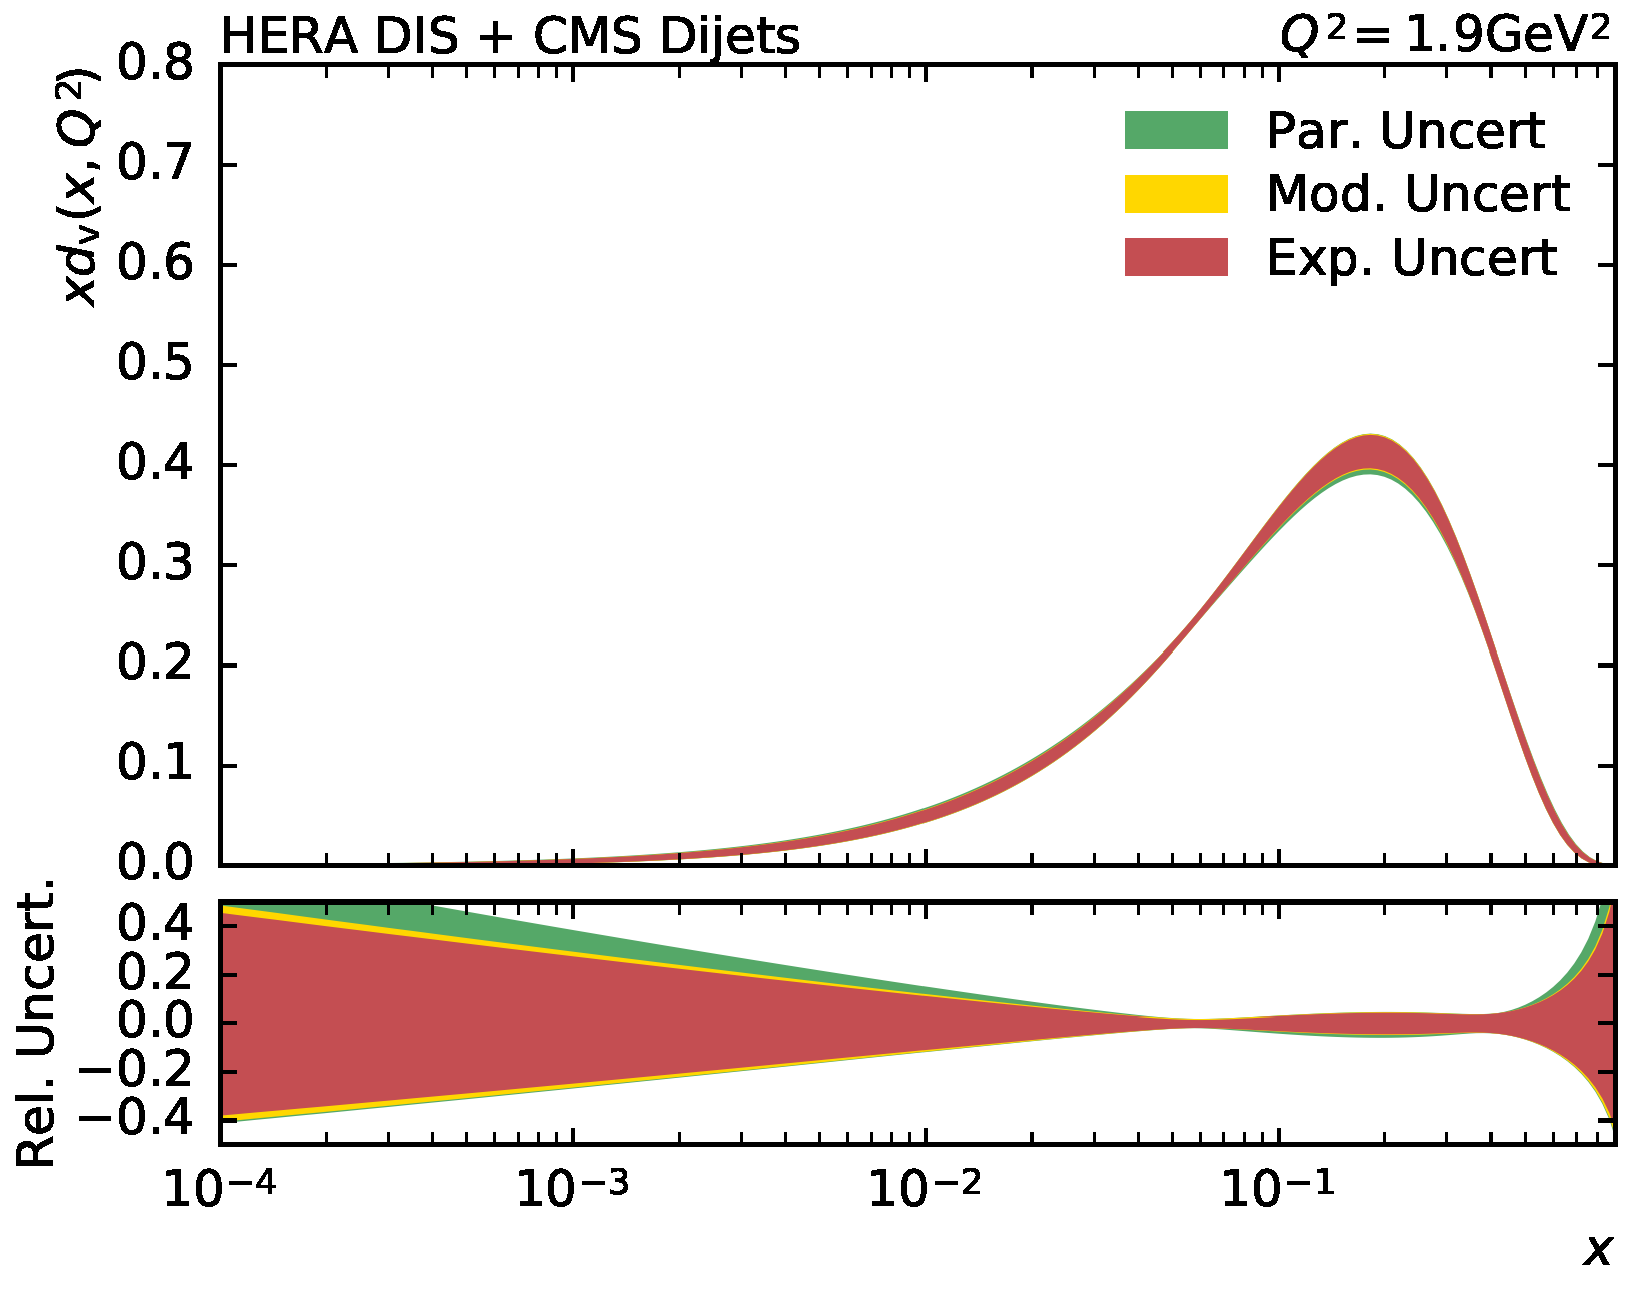
\includegraphics[width=0.48\textwidth]{figures/pdf_constraints/pdfcomp_HFTD_HERACMSTDJETS_7_1.9.pdf}
  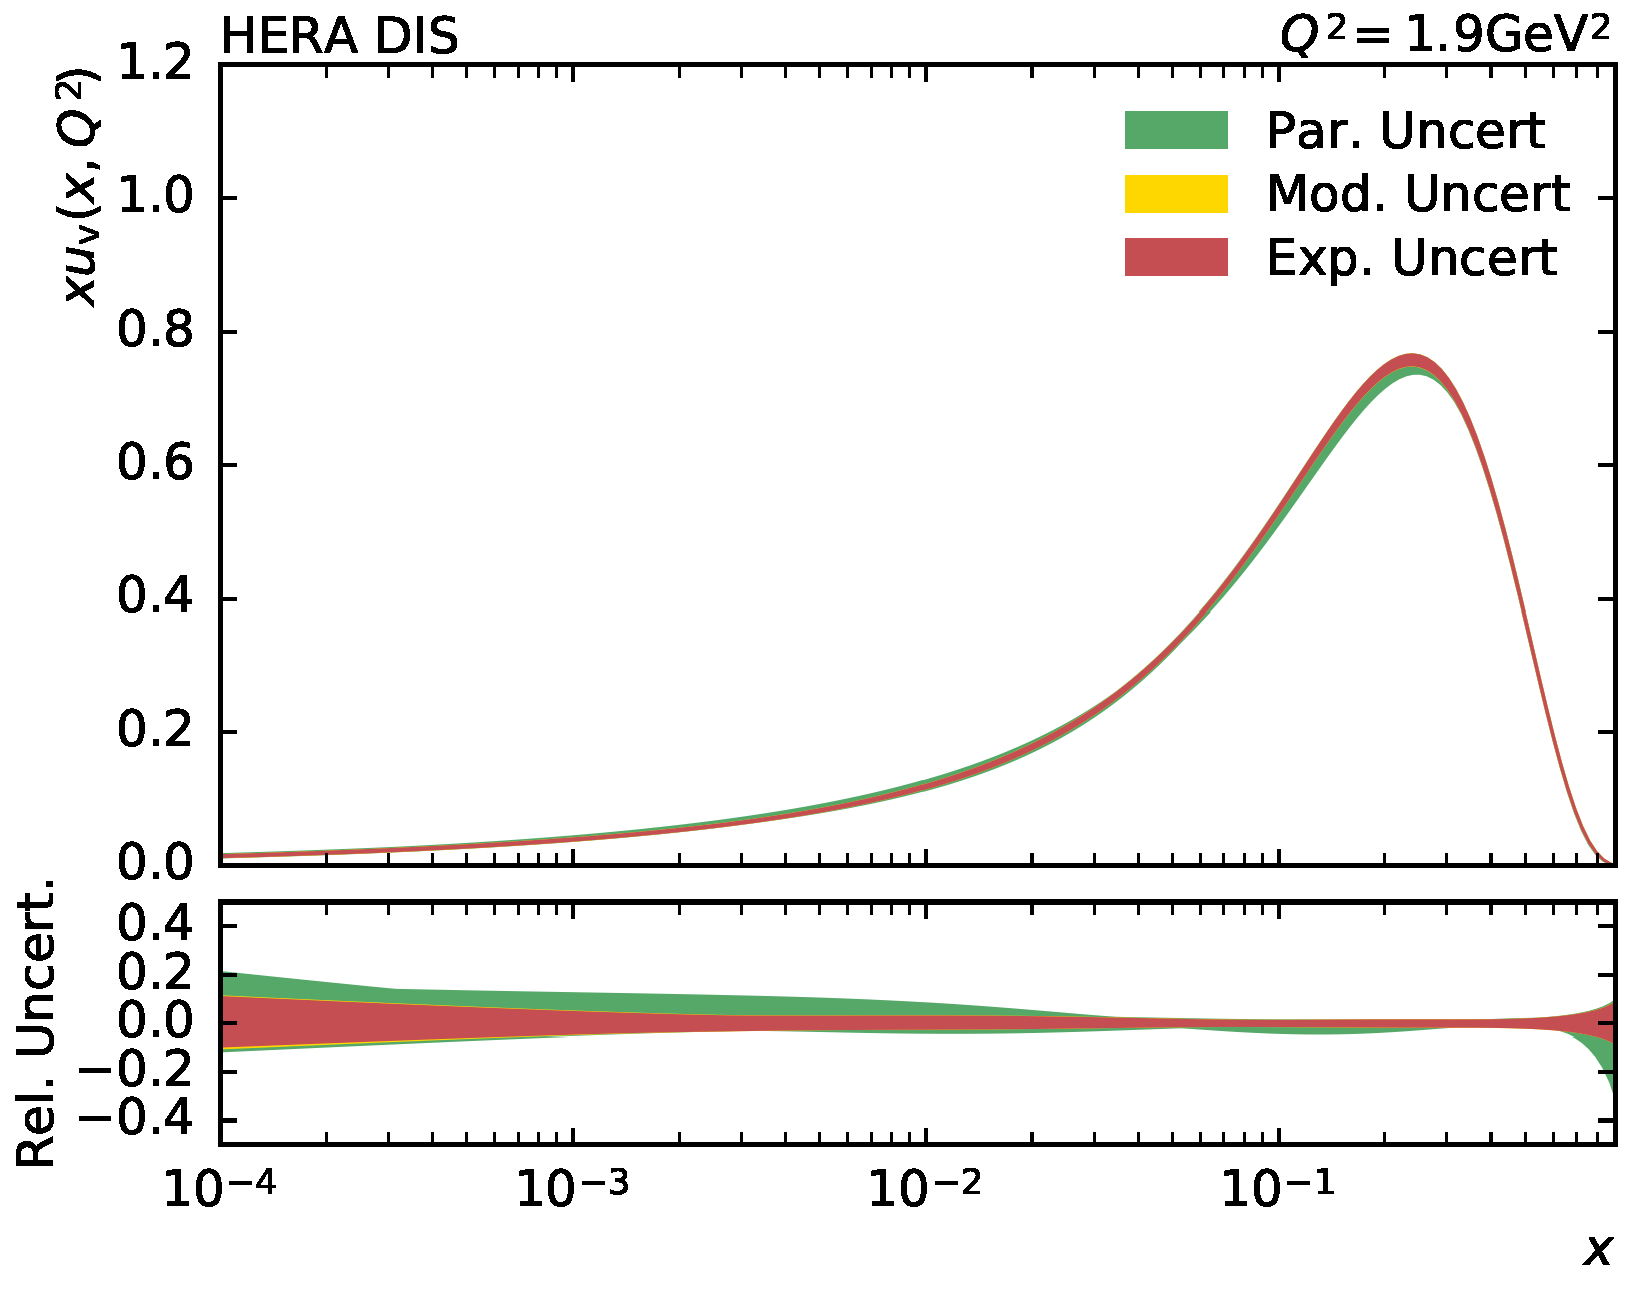
\includegraphics[width=0.48\textwidth]{figures/pdf_constraints/pdfcomp_HFTD_HERA_8_1.9.pdf}\hfill%
  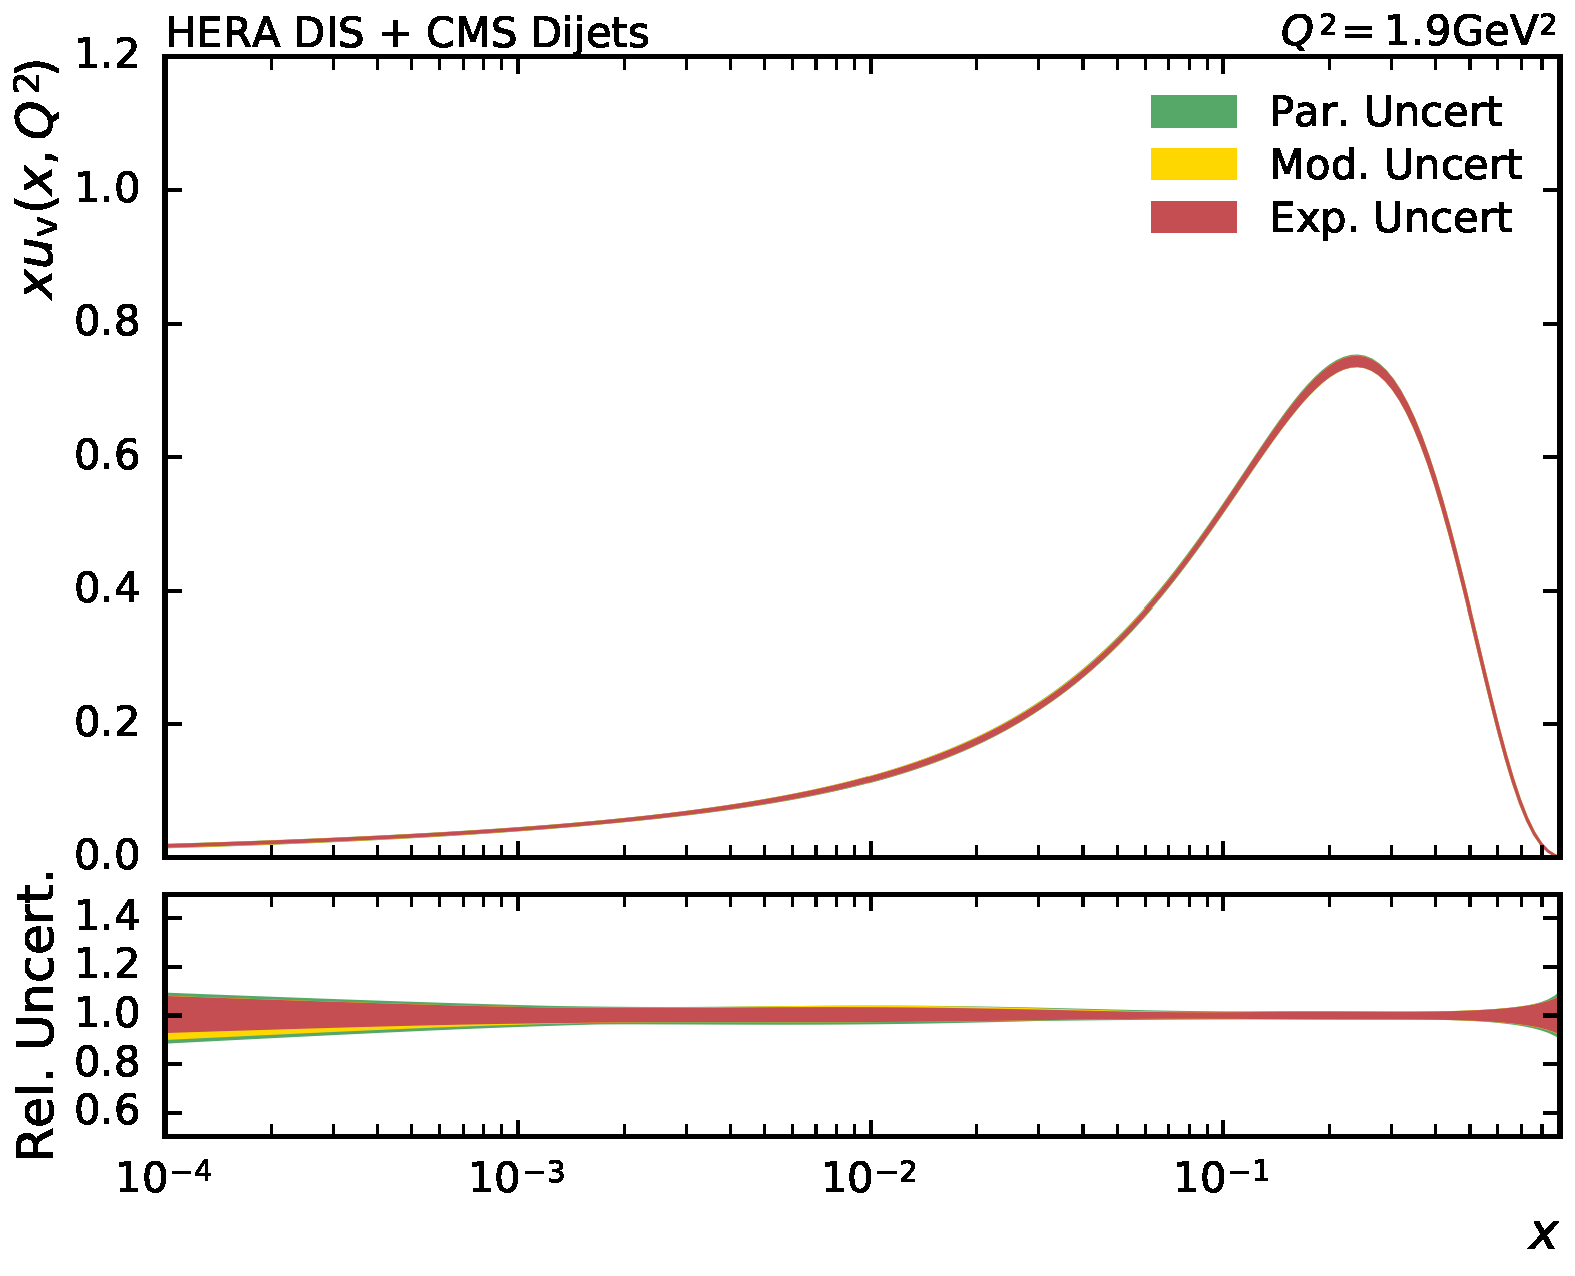
\includegraphics[width=0.48\textwidth]{figures/pdf_constraints/pdfcomp_HFTD_HERACMSTDJETS_8_1.9.pdf}

  \caption[The d valence and u valence quark PDFs]{The d valence quark (top) and u
    valence quark (bottom) PDFs as a function of $x$ as
  derived from HERA inclusive DIS data alone (left) and in combination with
  the CMS dijet data (right). The PDFs are shown at the starting scale $Q^2 =
  \SI{1.9}{\GeV \squared}$. The experimental (inner band), model (middle band)
  and parametrization uncertainties (outer band) are added quadratically to give
  the total uncertainty.}
  \label{fig:pdfconstraints:split:dvaluval:19}
\end{figure}


\begin{figure}[tbp]
  \centering
  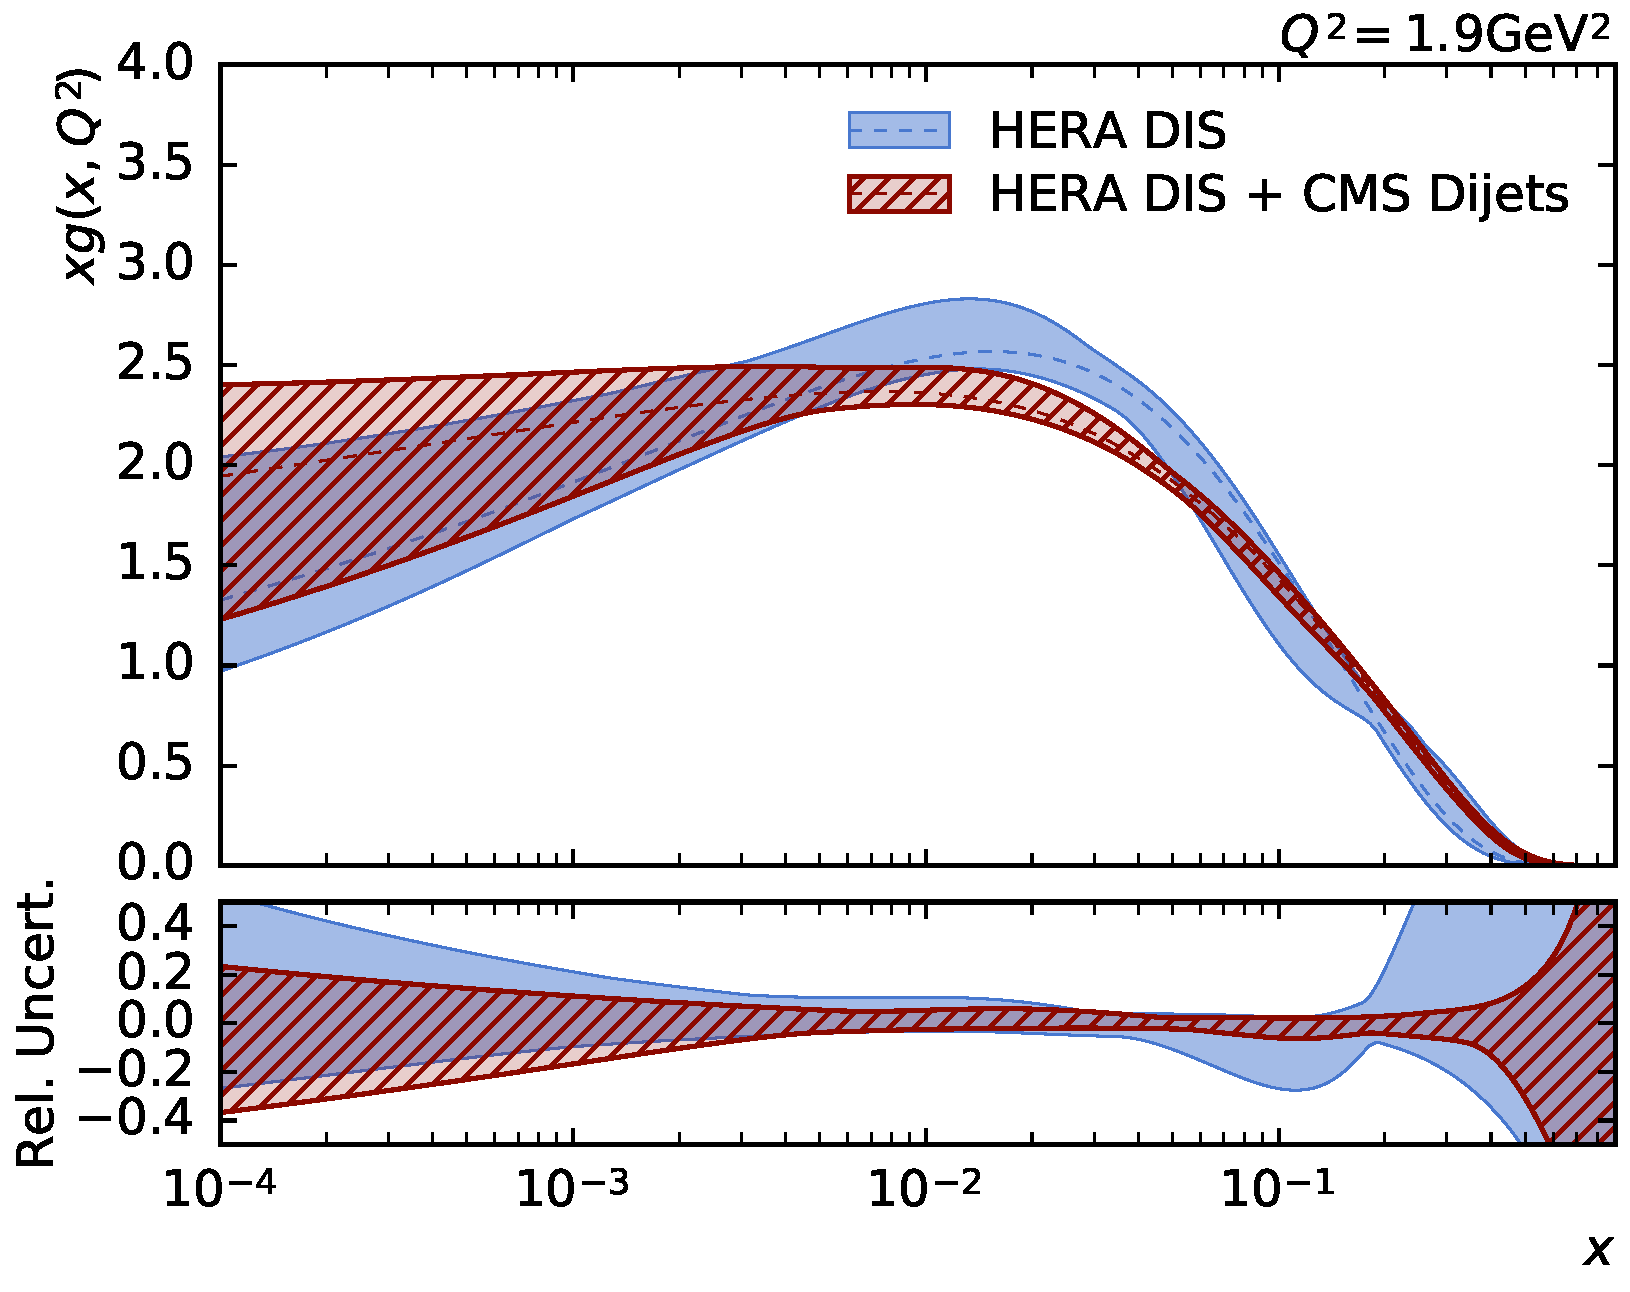
\includegraphics[width=0.48\textwidth]{figures/pdf_constraints/pdfcomp_direct_0_1.9.pdf}\hfill%
  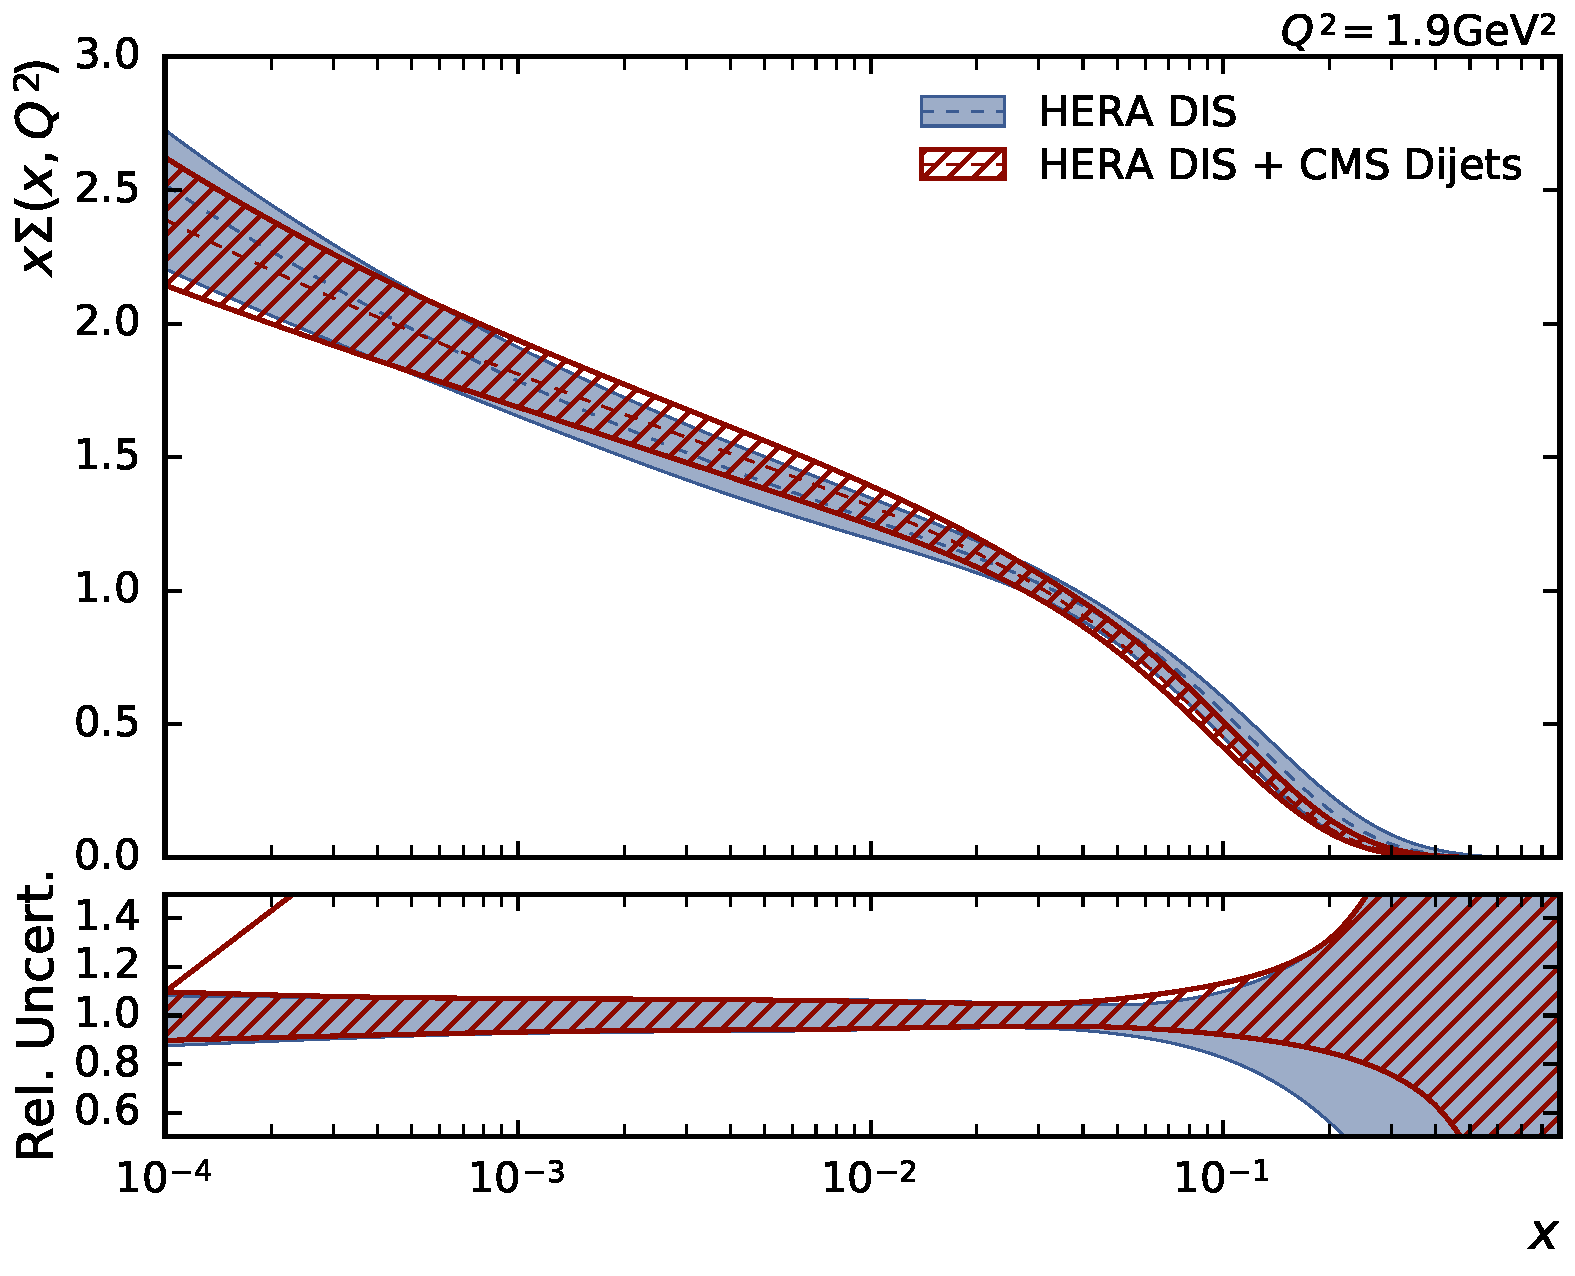
\includegraphics[width=0.48\textwidth]{figures/pdf_constraints/pdfcomp_direct_9_1.9.pdf}
  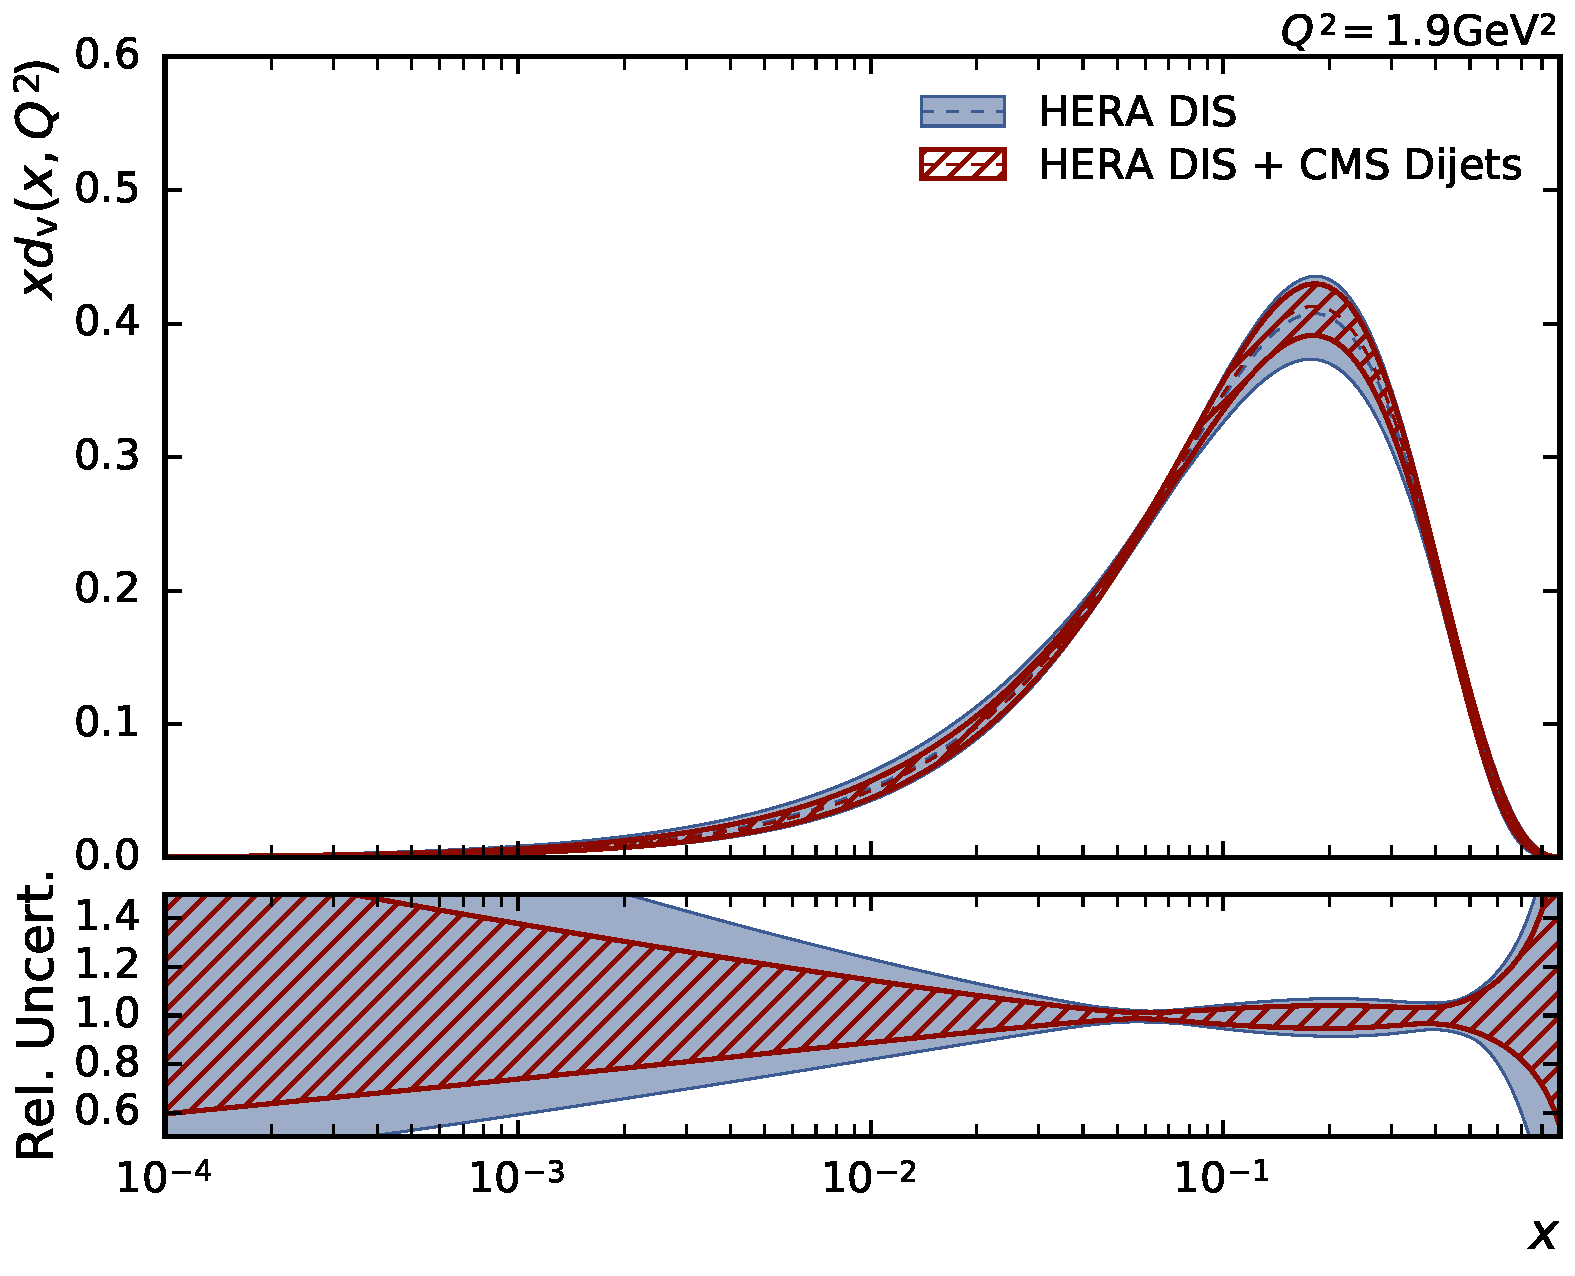
\includegraphics[width=0.48\textwidth]{figures/pdf_constraints/pdfcomp_direct_7_1.9.pdf}\hfill%
  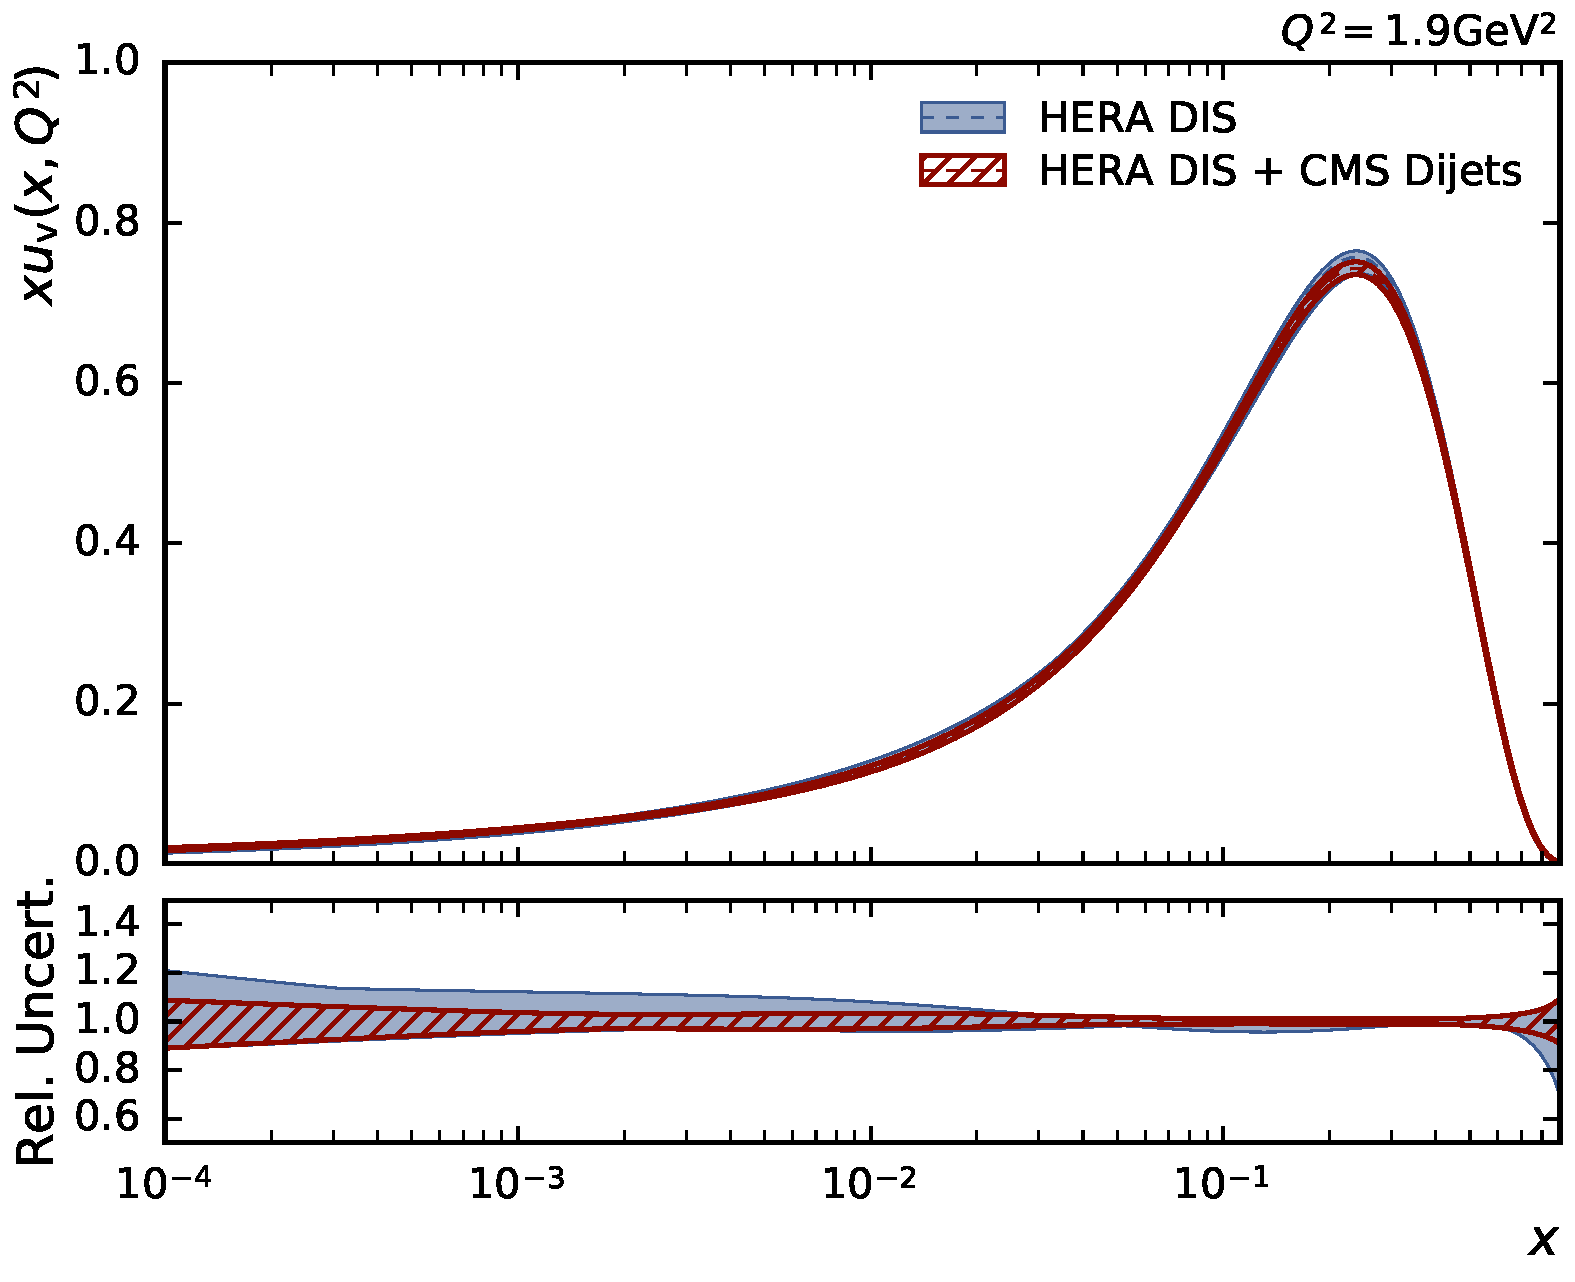
\includegraphics[width=0.48\textwidth]{figures/pdf_constraints/pdfcomp_direct_8_1.9.pdf}
  \caption[Direct comparison of gluon and quark PDFs]{The gluon (top left), sea
  quark (top right), d valence quark (bottom left) and u valence quark (bottom
right) PDFs as a function of $x$ as derived from HERA inclusive DIS data
alone (hatched band) and in combination with CMS dijet data (solid band). The PDFs
are shown at the starting scale $Q^2 = \SI{1.9}{\GeV \squared}$. The total
uncertainty of the PDFs is shown.}
  \label{fig:pdfconstraints:direct:19}
\end{figure}


\begin{figure}[tbp]
  \centering
  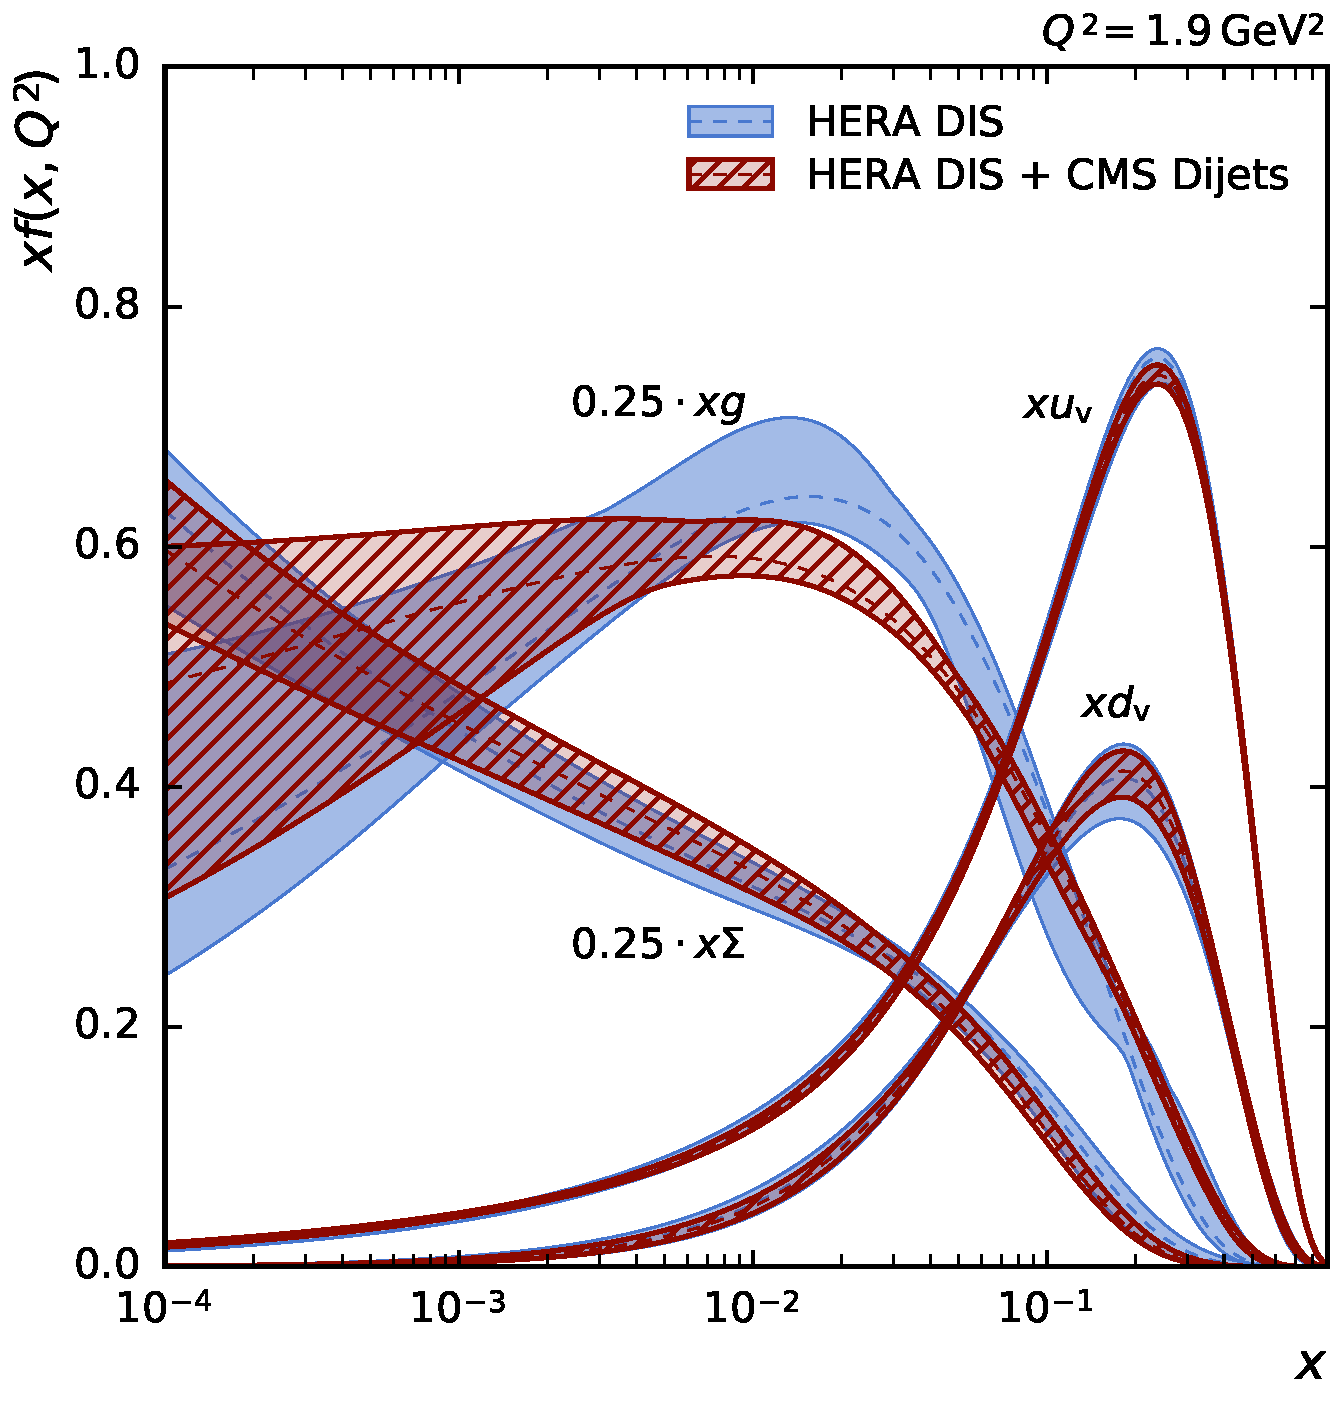
\includegraphics[width=0.7\textwidth]{figures/pdf_constraints/pdfcomp_direct_overview_1.9.pdf}\hfill%
  \caption[Overview of gluon and quark PDFs]{Overview of the gluon, sea, u
  valence and d valence quark PDFs before (hatched band) and after (solid band)
  including the CMS dijet data in the fit. The PDFs are shown at the starting
  scale $Q^2 = \SI{1.9}{\GeV \squared}$. The PDFs are shown with total
  uncertainties.}
  \label{fig:pdfconstraints:overview:19}
\end{figure}

\section{Simultaneous Fit of PDFs and Strong Coupling Constant}

The triple-differential dijet cross section does not only provide constraints on
the PDFs, but also on the strong coupling constant. The bin which contains the
boosted dijet events is the most sensitive to the PDFs. However, the
experimental uncertainties are larger than in the bin containing two central
jets, \ie at low \yboost and low \ystar values. At the same time, the highest
transverse momentum are reached in that bin. Due to the known correlations
between these phase space regions, this measurement is a good input for a
simultaneous fit of both the PDFs and the strong coupling. 

Therefore, the same PDF fit as in the previous section is performed but with the
additional free parameter \as. The uncertainty on \as is determined using
\textsc{Minuit} by profiling the likelihood. Furthermore, the model and
parameterization uncertainties were calculated in the same way as in
Sec.~\ref{section:cmsjets2011_pdfconstraints}. In addition, the scale
uncertainties are estimated by varying the renormalization and factorization
scale and repeating the fit in a similar way as in
Sec.~\ref{sec:scale_uncertainties}. The scale of the HERA DIS remained
unchanged. 
\todo{add scale uncertainties from fixed PDFs}

The strong coupling constant \asmz is determined as

\begin{equation*}
  \asmz = 0.1188_{-0.0015}^{+0.0015}(\mathrm{exp})_{-0.0002}^{+0.0004}(\mathrm{mod})_{-0.0005}^{+0.0003}(\mathrm{par})_{-0.0010}^{+0.0029}(\mathrm{scale})
\end{equation*}

where the \emph{exp} uncertainty accounts for the experimental uncertainties of
the incvlusive HERA DIS and CMS jet data and NP uncertainties. The \emph{mod}
and \emph{par} uncertainty denotes the model respectively the parameterization
uncertainty and \emph{scale} the scale uncertainties.  The determined value of
\asmz in agreement with the world average of $\asmz=0.1181\pm 0.0013$ of the
PDG~\cite{Agashe:2014kda}.
\todo{rewrite paragraph}
